%-------------------------------------------------------------------------------
%	PACKAGES AND OTHER DOCUMENT CONFIGURATIONS
%-------------------------------------------------------------------------------

\documentclass[
11pt, % The default document font size, options: 10pt, 11pt, 12pt
%oneside, % Two side (alternating margins) for binding by default, uncomment to switch to one side
english, % ngerman for German
singlespacing, % Single line spacing, alternatives: onehalfspacing or doublespacing
%draft, % Uncomment to enable draft mode (no pictures, no links, overfull hboxes
%indicated) nolistspacing, % If the document is onehalfspacing or doublespacing,
%uncomment this to set spacing in lists to single liststotoc, % Uncomment to add
%the list of figures/tables/etc to the table of contents toctotoc, % Uncomment
%to add the main table of contents to the table of contents parskip, % Uncomment
%to add space between paragraphs nohyperref, % Uncomment to not load the
%hyperref package
headsepline, % Uncomment to get a line under the header
%chapterinoneline, % Uncomment to place the chapter title next to the number on one line
%consistentlayout, % Uncomment to change the layout of the declaration, abstract and acknowledgements pages to match the default layout
]{MastersThesis} % The class file specifying the document structure

\usepackage[utf8]{inputenc} % Required for inputting international characters
\usepackage[T1]{fontenc} % Output font encoding for international characters

\usepackage{mathpazo} % Use the Palatino font by default
\usepackage{tikz}
\usepackage{acronym} % Acronyms
\usetikzlibrary{decorations.pathreplacing,positioning, arrows.meta}
\newcommand{\ImageWidth}{11cm}
\definecolor{myLightGray}{RGB}{191,191,191}
\definecolor{myGray}{RGB}{160,160,160}
\definecolor{myDarkGray}{RGB}{144,144,144}
\definecolor{myDarkRed}{RGB}{167,114,115}
\definecolor{myRed}{RGB}{255,58,70}
\definecolor{myGreen}{RGB}{0,255,71}
\usepackage{hyperref}
\usepackage{parskip}
\usepackage{algorithm}
\usepackage{algpseudocode}
\usepackage{etoolbox}
\usepackage{enumitem}
\usepackage[most]{tcolorbox}
\usepackage{siunitx}
\DeclareSIUnit{\voltpeak}{Vp}
\usepackage{svg}
\usepackage{tikz-3dplot}
\usepackage[a]{esvect}
\usepackage{lipsum}
\usepackage{amsthm}
\usepackage{etoolbox} % for patching
\tcbuselibrary{theorems}
\usetikzlibrary{arrows.meta, positioning}


% REFs/Citations/Acronyms/Links blue

% Define boxed definition environment with no rounded corners
\tcolorboxenvironment{definition}{
  enhanced,
  colback=red!5,            % light red background
  boxrule=0pt,            % border thickness
  arc=0mm,                  % no rounded corners
  sharp corners,            % enforce sharp edges
  top=0mm,
  bottom=1mm,
  left=2mm,
  right=2mm,
  before skip=10pt,
  after skip=10pt
}
\tcolorboxenvironment{theorem}{
  enhanced,
  colback=gray!10,        % light grey background
  boxrule=0pt,            % no border
  arc=0mm,
  sharp corners,
  top=0mm,
  bottom=1mm,
  left=2mm,
  right=2mm,
  before skip=10pt,
  after skip=10pt
}

\theoremstyle{definition}
\newtheorem{definition}{Definition}[section]
\theoremstyle{plain}
\newtheorem{theorem}[definition]{Theorem}
\makeatletter
\patchcmd{\@begintheorem}{\ignorespaces}{\vspace{1em}\ignorespaces}{}{}
\patchcmd{\@opargbegintheorem}{\ignorespaces}{\vspace{1em}\ignorespaces}{}{}
\patchcmd{\@endtheorem}{\unskip}{\unskip\vspace{1em}}{}{}
\makeatother

\theoremstyle{remark}
\newtheorem{remark}[definition]{Remark}
\theoremstyle{remark}
\newtheorem{example}[definition]{Example}

\usetikzlibrary{decorations.pathmorphing} % for zigzag


% Linecomments in algorithms
\usepackage{xcolor}
\newcommand{\commentsymbol}{\textcolor{green!50!black}{//}}% or \% or $\triangleright$
\algrenewcommand\algorithmiccomment[1]{\hfill {\color{green!50!black}\commentsymbol{} #1}}
\makeatletter
\newcommand{\LineComment}[2][\algorithmicindent]{\Statex \hspace{#1}{\color{green!50!black}\commentsymbol{} #2}}
\makeatother
\newcommand{\varfont}{\texttt}

% \usepackage{cleveref}

\hypersetup{
    colorlinks=true,
    linkcolor=blue,
    filecolor=magenta,      
    urlcolor=cyan,
    pdftitle={Overleaf Example},
    pdfpagemode=FullScreen,
    citecolor=blue
}

\usepackage[backend=bibtex,natbib=true]{biblatex} % Use the bibtex backend with the authoryear citation style (which resembles APA)

\addbibresource{example.bib} % The filename of the bibliography

\usepackage[autostyle=true]{csquotes} % Required to generate language-dependent quotes in the bibliography

%----------------------------------------------------------------------------------------
%	MARGIN SETTINGS
%----------------------------------------------------------------------------------------

\geometry{
	paper=a4paper, % Change to letterpaper for US letter
	inner=2.5cm, % Inner margin
	outer=3.8cm, % Outer margin
	bindingoffset=.5cm, % Binding offset
	top=1.5cm, % Top margin
	bottom=1.5cm, % Bottom margin
	head=27.2pt, % Adjust head height to avoid warnings
	%showframe, % Uncomment to show how the type block is set on the page
}

%----------------------------------------------------------------------------------------
%	THESIS INFORMATION
%----------------------------------------------------------------------------------------

\thesistitle{Quasi-Monte Carlo Methods and Applications} % Your thesis title, this is used in the title and abstract, print it elsewhere with \ttitle
\supervisor{Prof. Dr. Andreas \textsc{Neuenkirch}} % Your supervisor's name, this is used in the title page, print it elsewhere with \supname
\examiner{} % Your examiner's name, this is not currently used anywhere in the template, print it elsewhere with \examname
\degree{Master of Science} % Your degree name, this is used in the title page and abstract, print it elsewhere with \degreename
\author{Janik V. \textsc{Hrubant}} % Your name, this is used in the title page and abstract, print it elsewhere with \authorname
\addresses{} % Your address, this is not currently used anywhere in the template, print it elsewhere with \addressname

\subject{Mathematics} % Your subject area, this is not currently used anywhere in the template, print it elsewhere with \subjectname
\keywords{} % Keywords for your thesis, this is not currently used anywhere in the template, print it elsewhere with \keywordnames
\university{\href{https://www.uni-mannheim.de/en/}{University of Mannheim}} % Your university's name and URL, this is used in the title page and abstract, print it elsewhere with \univname
\department{\href{http://department.university.com}{Department or School Name}} % Your department's name and URL, this is used in the title page and abstract, print it elsewhere with \deptname
\group{\href{http://researchgroup.university.com}{Research Group Name}} % Your research group's name and URL, this is used in the title page, print it elsewhere with \groupname
\faculty{\href{http://faculty.university.com}{Faculty Name}} % Your faculty's name and URL, this is used in the title page and abstract, print it elsewhere with \facname

\AtBeginDocument{
\hypersetup{pdftitle=\ttitle} % Set the PDF's title to your title
\hypersetup{pdfauthor=\authorname} % Set the PDF's author to your name
\hypersetup{pdfkeywords=\keywordnames} % Set the PDF's keywords to your keywords
}

\begin{document}

\frontmatter % Use roman page numbering style (i, ii, iii, iv...) for the pre-content pages

\pagestyle{plain} % Default to the plain heading style until the thesis style is called for the body content

%----------------------------------------------------------------------------------------
%	TITLE PAGE
%----------------------------------------------------------------------------------------

\begin{titlepage}
\begin{center}

\vspace*{.06\textheight}
{\scshape\LARGE \univname\par}\vspace{1.5cm} % University name
\textsc{\Large Master Thesis}\\[0.5cm] % Thesis type

\HRule \\[0.4cm] % Horizontal line
{\huge \bfseries \ttitle\par}\vspace{0.4cm} % Thesis title
\HRule \\[1.5cm] % Horizontal line
 
\begin{minipage}[t]{0.4\textwidth}
\begin{flushleft} \large
\emph{Author:}\\
\authorname % Author name - remove the \href bracket to remove the link
\end{flushleft}
\end{minipage}
\begin{minipage}[t]{0.4\textwidth}
\begin{flushright} \large
\emph{Supervisors:} \\
\supname % Supervisor name - remove the \href bracket to remove the link  
\end{flushright}
\end{minipage}\\[3cm]
 
\vfill

\large \textit{A thesis submitted in fulfillment of the requirements\\ for the degree of \degreename}\\[0.3cm] % University requirement text
\textit{in the}\\[0.4cm]
\groupname\\\deptname\\[2cm] % Research group name and department name
 
\vfill

{\large \today}\\[4cm] % Date
%\includegraphics{Logo} % University/department logo - uncomment to place it
 
\vfill
\end{center}
\end{titlepage}

%----------------------------------------------------------------------------------------
%	DECLARATION PAGE
%----------------------------------------------------------------------------------------

\begin{declaration}
\addchaptertocentry{\authorshipname} % Add the declaration to the table of contents

\paragraph{English Version.} I hereby declare that I have completed this thesis
independently and without any unauthorized assistance. I further confirm that
neither this thesis nor any part of it has been submitted by me or by others as
part of any other academic assessment. Literal or paraphrased quotations from
other sources—whether in print or electronic form—are clearly marked as such.
All secondary literature and other sources used are properly cited and listed in
the bibliography. This also applies to graphical representations, images, and
all online sources. I furthermore agree that my thesis may be submitted and
stored in anonymized electronic form for the purpose of plagiarism detection. I
am aware that the thesis may not be evaluated if this declaration is not
submitted.

\paragraph{German Version.} Hiermit versichere ich, dass diese Arbeit von mir
persönlich verfasst wurde und dass ich keinerlei fremde Hilfe in Anspruch
genommen habe. Ebenso versichere ich, dass diese Arbeit oder Teile daraus weder
von mir selbst noch von anderen als Leistungsnachweise andernorts eingereicht
wurden. Wörtliche oder sinngemäße Übernahmen aus anderen Schriften und
Veröffentlichungen in gedruckter oder elektronischer Form sind gekennzeichnet.
Sämtliche Sekundärliteratur und sonstige Quellen sind nachgewiesen und in der
Bibliographie aufgeführt. Das Gleiche gilt für graphische Darstellungen und
Bilder sowie für alle Internet-Quellen. Ich bin ferner damit einverstanden, dass
meine Arbeit zum Zwecke eines Plagiatsabgleichs in elektronischer Form
anonymisiert versendet und gespeichert werden kann. Mir ist bekannt, dass von
der Korrektur der Arbeit abgesehen werden kann, wenn diese Erklärung nicht
erteilt wird.
\vspace{1.5cm}

\begin{flushleft}
  \begin{minipage}[t]{0.5\textwidth}
    \noindent\rule[0.5em]{18em}{0.5pt} \\[0em] % Line for place and date
    Place, Date
  \end{minipage}%
  \begin{minipage}[t]{0.45\textwidth}
    \raggedleft
    \noindent\rule[0.5em]{12em}{0.5pt} \\[0em] % Line for signature
    Signature
  \end{minipage}
\end{flushleft}
\end{declaration}

\cleardoublepage

%-------------------------------------------------------------------------------
%	QUOTATION PAGE
%-------------------------------------------------------------------------------

% \vspace*{0.2\textheight}

% \noindent\enquote{\itshape Thanks to my solid academic training, today I can write hundreds of words on virtually any topic without possessing a shred of information, which is how I got a good job in journalism.}\bigbreak

% \hfill Dave Barry

%-------------------------------------------------------------------------------
%	ABSTRACT PAGE
%-------------------------------------------------------------------------------d

\begin{abstract}
\addchaptertocentry{\abstractname}
Here comes the Abstract or Introduction of the thesis.
\end{abstract}

%-------------------------------------------------------------------------------
%	ACKNOWLEDGEMENTS
%-------------------------------------------------------------------------------

% \begin{acknowledgements}
% \addchaptertocentry{\acknowledgementname} % Add the acknowledgements to the table of contents
% The acknowledgments and the people to thank go here, don't forget to include your project advisor\ldots
% \end{acknowledgements}

%-------------------------------------------------------------------------------
%	LIST OF CONTENTS/FIGURES/TABLES PAGES
%-------------------------------------------------------------------------------

\tableofcontents % Prints the main table of contents

% \listoffigures % Prints the list of figures

% \listoftables % Prints the list of tables

%-------------------------------------------------------------------------------
%	ABBREVIATIONS
%-------------------------------------------------------------------------------

\newpage
\begin{acronym}
\acro{rita}[RITA]{Rational Inverse Transform with Aliasing}
\acro{cdf}[CDF]{Cumulative Distribution Function}
\acro{qmc}[QMC]{Quasi-Monte Carlo}
\acro{mc}[MC]{Monte Carlo}
\acro{hu}[HU]{Hounsfield Unit}
\acro{ct}[CT]{Computed Tomography}
\acro{cbct}[CBCT]{Cone-Beam Computed Tomography}
\acro{ffd}[FFD]{Forced Fixed Detection}
\acro{cnn}[CNN]{Convolutional Neural Network}
\acro{dnn}[DNN]{Deep Neural Network}
\acro{pde}[PDE]{Partial Differential Equation}
\end{acronym}

%-------------------------------------------------------------------------------
%	PHYSICAL CONSTANTS/OTHER DEFINITIONS
%-------------------------------------------------------------------------------

% \begin{constants}{lr@{${}={}$}l} % The list of physical constants is a three column table

% % The \SI{}{} command is provided by the siunitx package, see its documentation for instructions on how to use it

% Speed of Light & $c_{0}$ & \SI{2.99792458e8}{\meter\per\second} (exact)\\
% %Constant Name & $Symbol$ & $Constant Value$ with units\\

% \end{constants}

%-------------------------------------------------------------------------------
%	SYMBOLS
%-------------------------------------------------------------------------------

% \begin{symbols}{lll} % Include a list of Symbols (a three column table)

% $a$ & distance & \si{\meter} \\
% $P$ & power & \si{\watt} (\si{\joule\per\second}) \\
% %Symbol & Name & Unit \\

% \addlinespace % Gap to separate the Roman symbols from the Greek

% $\omega$ & angular frequency & \si{\radian} \\

% \end{symbols}

%-------------------------------------------------------------------------------
%	ACRONYMS
%-------------------------------------------------------------------------------

\acro{rita}[RITA]{Rational Inverse Transform with Aliasing}
\acro{cdf}[CDF]{Cumulative Distribution Function}
\acro{qmc}[QMC]{Quasi-Monte Carlo}
\acro{mc}[MC]{Monte Carlo}
\acro{hu}[HU]{Hounsfield Unit}
\acro{ct}[CT]{Computed Tomography}
\acro{cbct}[CBCT]{Cone-Beam Computed Tomography}
\acro{ffd}[FFD]{Forced Fixed Detection}
\acro{cnn}[CNN]{Convolutional Neural Network}
\acro{dnn}[DNN]{Deep Neural Network}
\acro{pde}[PDE]{Partial Differential Equation}

%-------------------------------------------------------------------------------
%	DEDICATION
%-------------------------------------------------------------------------------

% \dedicatory{For/Dedicated to/To my\ldots} 

%-------------------------------------------------------------------------------
%	THESIS CONTENT - CHAPTERS
%-------------------------------------------------------------------------------

\mainmatter % Begin numeric (1,2,3...) page numbering

\pagestyle{thesis} % Return the page headers back to the "thesis" style

% Include the chapters of the thesis as separate files from the Chapters folder
% Uncomment the lines as you write the chapters

%!TEX root = ../main.tex
\part{Fundamentals of Quasi-Monte Carlo Methods}
\label{part1}

\chapter{Monte Carlo and Quasi-Monte Carlo Integration}
\label{chapter1}

% ------------------------------------------------------------------------------
% ------------------------------------------------------------------------------
\section{Motivation and Problem Setting}
% ------------------------------------------------------------------------------
% ------------------------------------------------------------------------------
The numerical evaluation of high-dimensional integrals is a fundamental task in
modern applied mathematics and scientific computing. Applications range from
Bayesian inference and financial mathematics to machine learning and
computational physics. In particular, contemporary domains such as deep neural
network training and medical imaging often require the estimation of integrals
of the form

\begin{equation}
    \label{eq:integration_problem}
    I(f) = \int_{[0,1]^s} f(x)\,dx\,,
\end{equation}

where $s$ denotes the dimensionality of the problem and $f$ is a function that
may be expensive or impractical to evaluate analytically.

One of the most widely used approaches to compute such integrals is the
classical \ac{mc} method, which estimates the expectation based on averages over
randomly sampled points. The primary appeal of \ac{mc} integration lies in its
dimension-independent convergence rate and minimal assumptions on the integrand.
However, its asymptotic error rate of $\mathcal{O}(N^{-1/2})$ limits its
efficiency -- especially when high precision is required or function evaluations
are computationally expensive.

\ac{qmc} methods offer an alternative paradigm: instead of random samples, they employ deterministic sequences -- so-called low-discrepancy sequences—that aim to fill the integration domain more uniformly. This structured sampling allows for faster convergence under certain smoothness conditions and forms the basis for many state-of-the-art techniques in high-dimensional numerical integration.

The goal of this part is to develop a rigorous mathematical foundation for
\ac{qmc} methods and to understand how they improve upon classical \ac{mc}
integration. The key concepts introduced here -- particularly discrepancy theory
and low-discrepancy sequences -- serve as theoretical tools that will be
revisited in later parts of this thesis. Chapter~\ref{chapter2} will delve into
the measurement of uniformity via star discrepancy and provide concrete
constructions of low-discrepancy sequences such as Sobol' and Halton, which are
central to the numerical methods applied in Part~\ref{part2} and
Part~\ref{part3}, dedicated to neural network training and CT-based photon
transport simulation.


% ------------------------------------------------------------------------------
\subsection{High-Dimensional Integration in Applications}
% ------------------------------------------------------------------------------
High-dimensional integration problems arise naturally in a wide range of
scientific and engineering disciplines. Whenever expectations with respect to
multivariate distributions must be computed numerically, they are typically
formulated as integrals over the $s$-dimensional unit cube -- such as the
integral in Equation~\eqref{eq:integration_problem}.

Prominent examples include:
\begin{itemize}
    \item \textbf{Bayesian statistics}: Computing posterior expectations, marginal likelihoods, or predictive distributions.
    \item \textbf{Financial mathematics}: Pricing complex financial derivatives and evaluating risk measures under stochastic models.
    \item \textbf{Machine learning}: Estimating expectations in variational inference, training neural networks using randomized optimization techniques, or evaluating generalization bounds.
    \item \textbf{Medical imaging}: Simulating photon transport and estimating physical quantities based on noisy measurements, especially in \ac{ct} and magnetic resonance imaging (MRI).
\end{itemize}

In all these cases, the dimensionality $s$ can be moderate to very high --
sometimes even exceeding hundreds or thousands of variables. This introduces
significant challenges for numerical integration methods, which must balance
accuracy, computational cost, and robustness with respect to the structure of
the integrand.

The remainder of this chapter explores how \ac{mc} and \ac{qmc} methods address
these challenges. Before doing so, we briefly review the \ac{mc} method and
its fundamental convergence properties in the next section.


% ------------------------------------------------------------------------------
\subsection{Monte Carlo Integration: Principle and Convergence}
% ------------------------------------------------------------------------------
The classical \ac{mc} method is a probabilistic approach to numerical
integration that relies on random sampling. It is particularly suited for
high-dimensional settings, as its convergence rate does not deteriorate with
increasing dimension.

\begin{definition}[Monte Carlo Estimator] \ \\
Let $f \in L^2([0,1]^s)$ and let $X_0, \dots, X_{N-1} \sim
\mathcal{U}([0,1]^s)$ be independent and identically distributed random samples.
The Monte Carlo estimator of the integral \( I \) is given by
\begin{equation}
    I_N^{\mathrm{MC}}(f) := \frac{1}{N} \sum_{n=0}^{N-1} f(X_n)\,.
\end{equation}
\end{definition}


This estimator is unbiased and converges almost surely to the true integral as $N \to \infty$, as established by the Strong Law of Large Numbers:

\begin{theorem}[Strong Law of Large Numbers] \ \\
Let $f \in L^2([0,1]^s)$. Then
\begin{equation}
\mathbb{P}\left[ \lim_{N \to \infty} I_N^{\mathrm{MC}}(f) = \int_{[0,1]^s} f(x)\, dx \right] = 1.
\end{equation}
\end{theorem}

Beyond this almost sure convergence, the expected integration error of the Monte
Carlo estimator can be quantified using the root-mean-square error \cite[Section 1.3]{pillichshammer2010zahlentheoretische}:

\begin{theorem}[Monte Carlo Convergence Rate] \ \\
\label{thm:mc-convergence-rate}
Let $f \in L^2([0,1]^s)$. Then
\begin{equation}
    \mathbb{E}\left[ \left| I_N^{\mathrm{MC}}(f) - I(f) \right| \right] \leq \frac{\sigma[f]}{\sqrt{N}},
\end{equation}
where $\sigma[f] := \sqrt{\mathrm{Var}[f]}$.
\end{theorem}

\begin{proof}[Sketch of Proof]
Using independence and linearity of expectation, the variance of $I_N^{\mathrm{MC}}(f)$ is
\begin{equation}
    \mathrm{Var}[I_N^{\mathrm{MC}}(f)] = \frac{\mathrm{Var}[f]}{N}.
\end{equation}
Applying Jensen's inequality yields the stated bound on the expected absolute error.
\end{proof}

\begin{remark}
The convergence rate $\mathcal{O}(N^{-1/2})$ is independent of the integration
dimension $s$, which is a key advantage of the \ac{mc} method. In contrast,
classical grid-based methods often suffer from the curse of dimensionality,
where the number of required samples grows exponentially with $s$.
\end{remark}

\begin{example}
Let $f \in C^1([0,1]^s)$ be a Lipschitz-continuous function. A uniform grid with
$N = m^s$ points has a worst-case error of $\mathcal{O}(N^{-1/s})$. In high
dimensions, this becomes prohibitively inefficient, while MC integration retains
the dimension-agnostic rate $\mathcal{O}(N^{-1/2})$. \cite[Section
1.1]{leobacher2014introduction}
\end{example}

Despite its robustness and simplicity, MC integration has several well-known limitations:
\begin{itemize}
    \item The convergence rate is relatively slow, especially for smooth integrands.
    \item Error bounds are probabilistic rather than deterministic.
    \item The method does not exploit structural properties of the integrand, such as smoothness or sparsity.
\end{itemize}

These limitations motivate the development of \ac{qmc} methods, which
will be introduced in the next section.


% ------------------------------------------------------------------------------
% ------------------------------------------------------------------------------
\section{Quasi-Monte Carlo Methods}
% ------------------------------------------------------------------------------
% ------------------------------------------------------------------------------

% ------------------------------------------------------------------------------
\subsection{Deterministic Sampling and Intuition}
% ------------------------------------------------------------------------------

Classical \ac{mc} methods approximate integrals over the unit cube $[0,1]^s$
using randomly sampled points. In contrast, \ac{qmc} methods replace
stochasticity with a deterministic strategy, aiming to cover the integration
domain in a more uniform and structured way.

\begin{definition}[Quasi-Monte Carlo Estimator] \ \\
Let $f \colon [0,1]^s \to \mathbb{R}$ be a measurable function and let
$\{\boldsymbol{x}_n\}_{n=1}^{N} \subset [0,1]^s$ be a deterministic point set.
Then the \emph{quasi-Monte Carlo estimator} for the integral
\begin{equation*}
    I(f) = \int_{[0,1]^s} f(\boldsymbol{x}) \, d\boldsymbol{x}
\end{equation*}
is defined as
\begin{equation}
I_N^{\mathrm{QMC}}(f) := \frac{1}{N} \sum_{n=1}^{N} f(\boldsymbol{x}_n).
\end{equation}
\end{definition}

The functions $I$, $I_N^{\mathrm{MC}}$ and $I_N^{\mathrm{QMC}}$ will be further
used without explicit reference to the integrand $f$ when the context is clear.

Unlike in the Monte Carlo setting, these points are not drawn from a probability
distribution, but are generated deterministically — typically by rules that aim
to avoid clustering and oversampling.

Figure~\ref{fig:mc-vs-qmc} illustrates this contrast by comparing $300$ randomly
sampled points to $300$ \ac{qmc} points from the Sobol' sequence in two
dimensions. The \ac{qmc} points distribute more evenly, avoiding both
gaps and clusters.

\begin{figure}[H]
  \centering
  \includegraphics[width=0.8\textwidth]{Figures/mc_vs_qmc.png}
  \caption{Comparison of $300$ sample points in $[0,1]^2$ using (left) standard 
  \ac{mc} and (right) a Sobol' sequence. \ac{qmc} points avoid clustering and 
  fill the domain more evenly.}
  \label{fig:mc-vs-qmc}
\end{figure}

A natural alternative to \ac{mc} sampling is the use of regular tensor-product
grids. However, these grids suffer from the \emph{curse of dimensionality}:
placing $m$ points per dimension leads to a total of $N = m^s$ points, which
becomes infeasible even for moderate $s$. Furthermore, grids are not easily
extensible -- adding new points requires global recomputation and destroys
nesting.

By contrast, many \ac{qmc} sequences, such as Sobol' and Halton (will be
introduced in Chapter~\ref{chapter2}), are designed to be \emph{incremental}:
each new point can be added without changing the existing ones. This makes
\ac{qmc} particularly suitable for adaptive algorithms, especially for anytime
algorithms that might increment the number of samples needed over time. However,
not all \ac{qmc} constructions share this feature such as lattice rules and some
optimized designs are fixed-size by nature.

\ac{qmc} methods thus offer the best of both worlds: they combine the
space-filling structure of grids with the flexibility and scalability of
sampling methods. Low-discrepancy sequences fill the space more evenly than
random points while avoiding the redundancy of regular grids. This often leads
to significantly lower integration errors, especially for smooth functions or
problems with low effective dimension.

This shift from probabilistic to deterministic sampling also changes the way we
analyze error: instead of using statistical bounds, we rely on \emph{discrepancy
measures}, which quantify the uniformity of the point set. These concepts, along
with the notion of function variation, will be introduced in the following
sections.

\begin{remark}
\ac{qmc} estimators retain the same algebraic structure as their \ac{mc}
counterparts, but their convergence behavior is governed by entirely different
theoretical tools -- namely discrepancy theory and function variation.
\end{remark}


% ------------------------------------------------------------------------------
\subsection{Monte Carlo vs. Quasi-Monte Carlo: A First Comparison}
\label{subsec:mc-vs-qmc}
% ------------------------------------------------------------------------------

\ac{mc} and \ac{qmc} methods share the same high-level goal: estimating an
integral by averaging function evaluations at selected sample points. The
difference lies in the sampling strategy -- stochastic versus deterministic --
and the consequences this has for accuracy, convergence and theoretical
guarantees.

Table~\ref{tab:mc-vs-qmc} summarizes key conceptual distinctions between the two paradigms.

\begin{table}[H]
\centering
\resizebox{0.95\textwidth}{!}{
\renewcommand{\arraystretch}{1.4}
\begin{tabular}{l|c|c}
\textbf{Aspect} & \textbf{Monte Carlo (MC)} & \textbf{Quasi-Monte Carlo (QMC)} \\
\hline
Sampling & Independent random points & Deterministic low-discrepancy points \\
Error bounds & Probabilistic (in expectation) & Deterministic (worst-case) \\
Regularity assumptions on $f$ & Square integrability ($L^2$) & Bounded variation (HK) \\
Theoretical convergence & $\mathcal{O}(N^{-1/2})$ & Up to $\mathcal{O}(N^{-1})$ (heuristic) \\
Point extensibility & Trivial & Often supported (e.g., Sobol) \\
Robustness to noise & High & Low \\
\end{tabular}}
\caption{Conceptual comparison of \ac{mc} and \ac{qmc} integration methods.}
\label{tab:mc-vs-qmc}
\end{table}

While \ac{mc} estimators are unbiased and robust even under minimal assumptions,
their convergence is slow and does not improve when the integrand is smooth.
\ac{qmc} methods, on the other hand, exploit structure in the integrand -- such
as smoothness or low effective dimension -- and can yield significantly lower
integration errors.

However, \ac{qmc} methods lack probabilistic guarantees and depend more strongly
on the careful construction of the point set. Their performance can degrade if
the integrand exhibits high variability along many input dimensions or if the
chosen sequence is not well matched to the function.

The next subsection discusses the convergence rates of both methods in more
detail and highlights the interplay between dimensionality and integration
error.

% ------------------------------------------------------------------------------
\section{Uniformity Concepts}
\label{sec:uniformity-concepts}
% ------------------------------------------------------------------------------

The efficiency of \ac{qmc} methods hinges on how well the employed point sets
"fill" the integration domain $[0,1]^s$. This motivates the need for a precise
mathematical understanding of \emph{uniformity}. The present section introduces
two key concepts in this regard -- \emph{uniform distribution modulo one} and
\emph{equidistribution} -- and clarifies their relevance to numerical
integration.

% ------------------------------------------------------------------------------
\subsection{Uniform Distribution vs. Equidistribution}
% ------------------------------------------------------------------------------

While the terms \emph{uniform distribution} and \emph{equidistribution} are
sometimes used interchangeably in informal contexts, they carry distinct
meanings in the context of numerical integration. In \ac{qmc} methods, the
notion of \emph{uniform distribution modulo one} provides a rigorous criterion
for how evenly a sequence covers the unit cube. This concept forms the
foundation for analyzing the convergence behavior of QMC estimators.

\begin{definition}[Uniform Distribution Modulo One] \ \\
Let $(\boldsymbol{x}_n)_{n \in \mathbb{N}_0} \subset [0,1]^s$ be a sequence of
sample points. The sequence is said to be \emph{uniformly distributed modulo
one} (u.d.\ mod~1) if for every axis-aligned box $[\boldsymbol{a}
\boldsymbol{b}) \subset [0,1]^s$, the proportion of points falling into this box
converges to its Lebesgue measure:
\begin{equation*}
    \lim_{N \to \infty} \frac{1}{N} \sum_{n=0}^{N-1} \chi_{[\boldsymbol{a}, \boldsymbol{b})}(\boldsymbol{x}_n)
    = \lambda_s([\boldsymbol{a}, \boldsymbol{b})) \,,
\end{equation*}
where $\chi_A$ is the indicator function of the set $A$ and $\lambda_s$ denotes
the $s$-dimensional Lebesgue measure.
\end{definition}

This definition emphasizes asymptotic spatial coverage: in the limit, every
subregion of the domain is sampled proportionally to its volume. Importantly,
this property is purely deterministic and does not rely on any probabilistic
assumptions — in contrast to Monte Carlo methods, which only guarantee
uniformity in expectation.

In contrast, when speaking of a random sample $\{X_1, \dots, X_N\} \subset
[0,1]^s$ drawn independent and identically distributed (i.i.d.) from the uniform
distribution, we refer to a probabilistic concept of uniformity: each point is
independently drawn according to the uniform measure, but the empirical
distribution may not be uniformly spread in finite samples. Thus,
equidistribution refers to the ideal uniform coverage that we seek
deterministically, while uniform random sampling only ensures this behavior in
expectation or with high probability.

\begin{remark}
    Uniform distribution modulo one is a necessary condition for the convergence
    of \ac{qmc} estimators. If a point sequence is not u.d.\ mod 1, then there
    exists at least one Riemann-integrable function for which the sample average
    fails to converge to the integral.
\end{remark}

The following result, known as Weyl's criterion, provides a necessary and
sufficient condition for uniform distribution in terms of exponential sums. A
proof can be found in \cite{leobacher2014introduction}.

\begin{theorem}[Weyl's Criterion] \ \\
A sequence $(\boldsymbol{x}_n)_{n \geq 0} \subset [0,1)^s$ is uniformly distributed modulo one if and only if, for all nonzero $\boldsymbol{h} \in \mathbb{Z}^s \setminus \{\boldsymbol{0}\}$, we have
\begin{equation*}
    \lim_{N \to \infty} \frac{1}{N} \sum_{n=0}^{N-1} \exp(2\pi i\, \boldsymbol{h} \cdot \boldsymbol{x}_n) = 0.
\end{equation*}
\end{theorem}

\begin{example}
Let $\alpha \in \mathbb{R}$ be irrational. Then the Kronecker sequence $(n \alpha \bmod 1)_{n \geq 0}$ is uniformly distributed in $[0,1]$. This is a consequence of Weyl's criterion and illustrates the existence of simple, deterministic sequences with excellent uniformity properties.
\end{example}

% ------------------------------------------------------------------------------
\subsection{Why Uniformity Matters in Numerical Integration}
% ------------------------------------------------------------------------------

In \ac{qmc} integration, the objective is to approximate the integral defined in
Equation~\eqref{eq:integration_problem} by a finite average over a deterministic
point set $\{\boldsymbol{x}_0, \dots, \boldsymbol{x}_{N-1}\} \subset [0,1]^s$.
The accuracy of this approximation depends crucially on how uniformly the point
set samples the domain.

Unlike \ac{mc} methods, which rely on probabilistic guarantees and
variance-based error estimates, \ac{qmc} methods exploit deterministic
structure: the integration error is directly influenced by how well the point
set fills the domain. This insight gives rise to one of the most fundamental
theoretical tools in \ac{qmc} analysis: the \emph{Koksma--Hlawka inequality}.

\begin{remark}
The Koksma--Hlawka inequality bounds the integration error of a QMC estimator by
the product of two quantities: the \emph{star discrepancy} of the point set and
the \emph{variation} of the integrand in the sense of Hardy-Krause. In
short,
\begin{equation*}
    \left| \frac{1}{N} \sum_{n=0}^{N-1} f(\boldsymbol{x}_n) - I \right| 
    \leq D_N^*(\{\boldsymbol{x}_n\}) \cdot V_{\mathrm{HK}}(f).
\end{equation*}
A rigorous statement and detailed discussion of this inequality will follow in
Chapter~\ref{chapter3}.
\end{remark}

This inequality highlights why uniformity is essential: if the integrand has
bounded variation, then smaller discrepancy directly implies smaller integration
error. In this sense, discrepancy theory becomes a cornerstone of effective
\ac{qmc} integration.

\begin{remark}
The star discrepancy quantifies the maximal deviation between the empirical
distribution of the point set and the uniform distribution over $[0,1]^s$. It
vanishes asymptotically for uniformly distributed sequences and governs the
convergence behavior of \ac{qmc} estimators.
\end{remark}

The next chapter provides a formal introduction to discrepancy theory. We will
define extreme and star discrepancy, study their geometric interpretation, and
analyze the behavior of structured low-discrepancy sequences such as Halton and
Sobol'. These sequences, due to their uniform space-filling properties, play a
central role in modern high-dimensional numerical integration.

%!TEX root = ../main.tex
\chapter{Discrepancy Theory and Low-Discrepancy Sequences}
\label{chapter2}

% ------------------------------------------------------------------------------
\section{Measuring Uniformity: Discrepancy}
% ------------------------------------------------------------------------------

One of the cornerstones of \ac{qmc} theory is the concept of \emph{discrepancy},
which quantifies how uniformly a finite point set samples the $s$-dimensional
unit cube $[0,1]^s$. While uniform distribution modulo one describes the
asymptotic behavior of infinite sequences, discrepancy provides a finite-sample
measure of deviation from perfect uniformity. Low-discrepancy sequences are the
foundation of \ac{qmc} methods because they minimize this deviation and thus
yield more accurate numerical integration.

This section introduces formal definitions, geometric intuition and empirical
insights into discrepancy measures. It lays the theoretical groundwork for
understanding how the structure of point sets affects \ac{qmc} integration
performance.

% ------------------------------------------------------------------------------
\subsection{Definition of Discrepancy and Star Discrepancy}
% ------------------------------------------------------------------------------

First, we define the more general \emph{extreme discrepancy}:

\begin{definition}[Extreme Discrepancy] \ \\
Let $\mathcal{P}\subset [0,1)^s$, with $|\mathcal{P}| = N$, being a finite point
set. Then the extreme discrepancy $D_N(\mathcal{P})$ is defined as
\begin{equation*}
    D_N(\mathcal{P}) = \sup\limits_{\substack{\boldsymbol{a,b} \in [0,1]^s \\ \boldsymbol{a} \leq \boldsymbol{b}}} \bigg| \frac{A([\boldsymbol{a},\boldsymbol{b}) , \mathcal{P}, N)}{N} - \lambda_s([\boldsymbol{a},\boldsymbol{b})] \bigg|.
\end{equation*}
Hereby $A([\boldsymbol{a},\boldsymbol{b}), \mathcal{P}, N)$ denotes the number
of points in $\mathcal{P}$ that fall into the box
$[\boldsymbol{a},\boldsymbol{b})$, and
$\lambda_s([\boldsymbol{a},\boldsymbol{b})]$ is the Lebesgue measure of that
box, given by $\prod_{i=1}^{s} (b_i - a_i)$.
\end{definition}

In practice, a common and slightly more tractable variant is the \emph{star
discrepancy}, which restricts the test boxes to be anchored at the origin.

\begin{definition}[Star Discrepancy] \ \\
Let $\mathcal{P}\subset [0,1)^s$, with $|\mathcal{P}| = N$, being a finite point
set. Then the star discrepancy $D_N^*$ is defined as
\begin{equation*}
    D_N^*(\mathcal{P}) = \sup\limits_{\boldsymbol{t} \in [0,1]^s} \bigg| \frac{A([\boldsymbol{0},\boldsymbol{t}), \mathcal{P}, N)}{N} - \lambda_s([\boldsymbol{0},\boldsymbol{t})] \bigg|.
\end{equation*}
\end{definition}

This form is used in the Koksma--Hlawka inequality and serves as a central
measure in \ac{qmc} analysis. Note that both discrepancy definitions are
deterministic and depend solely on the point configuration.

\begin{remark}
A low star discrepancy implies that the empirical distribution of the points
approximates the uniform distribution well over all axis-aligned subrectangles
anchored at the origin.
\end{remark}

% ------------------------------------------------------------------------------
\subsection{Geometric Interpretation and Examples}
% ------------------------------------------------------------------------------

To build geometric intuition, consider the 1-dimensional case. Given $N$ sample
points $x_0, \dots, x_{N-1} \in [0,1)$, we can visualize discrepancy as the
maximum vertical deviation between the empirical distribution function
\begin{equation*}
F_N(t) := \frac{1}{N} \sum_{n=0}^{N-1} \chi_{[0,t)}(x_n)
\end{equation*}
and the uniform cumulative distribution function $F(t) = t$. The discrepancy
corresponds to the largest gap between $F_N(t)$ and $F(t)$.

In higher dimensions, the idea generalizes: the star discrepancy measures the
maximal difference in the number of points falling into an axis-aligned box
$[\boldsymbol{0}, \boldsymbol{t})$ versus the volume of that box. Intuitively,
it quantifies whether the point set "overpopulates" or "underpopulates" certain
regions.

\begin{figure}[H]
\centering
\includegraphics[scale=.67]{Figures/discrepancy1d.png}
\caption{Visualization of 1D discrepancy: the maximum vertical distance between the empirical CDF $F_N(t)$ and the uniform CDF $F(t) = t$.}
\label{fig:discrepancy-1d}
\end{figure}

\begin{example}
Let $x_n = \frac{n}{N}$ for $n = 0, \dots, N-1$. Then $F_N(t)$ is a
piecewise constant staircase function, and the discrepancy can be shown to be
$\mathcal{O}(1/N)$. This is an optimal rate in 1D.
\end{example}

\begin{remark}
Discrepancy provides a worst-case error metric over all subintervals. Thus, even
a point set that appears visually well-distributed may have large discrepancy
due to subtle gaps or clustering in certain regions.
\end{remark}

% ------------------------------------------------------------------------------
\subsection{Empirical Observation of Discrepancy in QMC}
% ------------------------------------------------------------------------------

Discrepancy is not just a theoretical construct -- its practical relevance
becomes evident when comparing the behavior of \ac{qmc} sequences with \ac{mc}
samples. In particular, structured point sets like Halton and Sobol' sequences
achieve much lower discrepancy than random samples of the same size.

\begin{figure}[H]
\centering
\includegraphics[width=0.9\textwidth]{Figures/qmc_discrepancy_comparison.png}
\caption{Comparison of discrepancy growth for Sobol', Halton and random
(\ac{mc}) point sets in 2D. Low-discrepancy sequences exhibit significantly
slower discrepancy growth.}
\label{fig:qmc-discrepancy-comparison}
\end{figure}

\begin{remark}
The expected star discrepancy of i.i.d. Monte Carlo samples decreases at the
rate $\mathcal{O}(N^{-1/2})$, whereas for low-discrepancy sequences, provable
upper bounds of order $\mathcal{O}((\log N)^s / N)$ exist.
\cite[Section~2.2]{leobacher2014introduction}
\end{remark}

The next section will introduce specific constructions of low-discrepancy
sequences and analyze their dimensional performance and implementation details.


% ------------------------------------------------------------------------------
\section{Construction of Low-Discrepancy Sequences}
% ------------------------------------------------------------------------------

Before defining specific low-discrepancy sequences, we first introduce the term of low-discrepancy sequences, which are designed to fill the unit cube $[0,1)^s$
as uniformly as possible.

\begin{definition}[Low-Discrepancy Sequence] \ \\
A sequence $\mathcal{S} = (x_n)_{n\in \mathbb{N}}$ in $[0,1)^s$ is called a low-discrepancy sequence if its star discrepancy satisfies
\begin{equation*}
    D_N^*(\mathcal{S}) = \mathcal{O}\left( \frac{(\log N)^s}{N} \right)
\end{equation*}
for all $N \in \mathbb{N}$. Such sequences are also referred to as
\emph{quasi-Monte Carlo sequences} or \ac{qmc} sequences.
\end{definition}

Low discrepancy sequences are constructed to minimize the star
discrepancy, which is crucial for the convergence of \ac{qmc} methods according to the Koksma-Hlawka inequality introduced in Chapter~\ref{chapter3}.

% ------------------------------------------------------------------------------
\subsection{The Halton Sequence}
\label{subsec:halton-sequence}
% ------------------------------------------------------------------------------

The Halton sequence is one of the earliest and most widely used constructions of
low-discrepancy sequences in arbitrary dimensions. 

For the construction of the Halton sequence, we utilize the radical-inverse
functin $\phi_b(n)$. The radical-inverse function $\phi_b(n)$ maps an integer
$n$ to a real number in $[0,1)$ by reflecting its base-$b$ representation about
the decimal point:
\begin{equation*}
    \phi_b(n) = \sum_{k=0}^\infty d_k b^{-k-1}, \quad \text{where } n = \sum_
    {k=0}^\infty d_k b^k.
\end{equation*}

\begin{definition}[Van der Corput Sequence] \ \\
\label{def:van-der-corput-sequence}
The one-dimensional van der Corput sequence in base $b$ is defined as
\begin{equation*}
    \mathcal{S}_b = \left( \phi_b(n) \right)_{n\in \mathbb{N}}.
\end{equation*}
\end{definition}

The Halton sequence generalizes the one-dimensional van der Corput sequence to
multiple dimensions by using mutually prime bases.

\begin{definition}[Halton Sequence] \ \\
Let $b_1, \dots, b_s$ be pairwise coprime integers greater than $1$, typically
chosen as the first $s$ prime numbers. The $n$-th point $\boldsymbol{x}_n \in
[0,1)^s$ of the $s$-dimensional Halton sequence is defined componentwise by
\begin{equation*}
    \boldsymbol{x}_n = \left( \phi_{b_1}(n), \dots, \phi_{b_s}(n) \right),
\end{equation*}
where $\phi_b(n)$ denotes the van der Corput radical-inverse function in base
$b$. The Halton sequence is then given by $\mathcal{S}_{b_1, \dots, b_s} = (x_n)_{n\in \mathbb{N}}$.
\end{definition}

\begin{example}[First Elements of the Halton Sequence in 2D] \ \\
Consider the two-dimensional Halton sequence based on the first two prime bases $b_1 = 2$ and $b_2 = 3$. The first three elements are obtained by computing the radical-inverse values $\phi_{b_1}(n)$ and $\phi_{b_2}(n)$ for $n = 1, 2, 3$:

\begin{itemize}
    \item $n = 1$: $\boldsymbol{x}_1 = \left( \phi_2(1), \phi_3(1) \right) = \left( \tfrac{1}{2}, \tfrac{1}{3} \right)$
    \item $n = 2$: $\boldsymbol{x}_2 = \left( \phi_2(2), \phi_3(2) \right) = \left( \tfrac{1}{4}, \tfrac{2}{3} \right)$
    \item $n = 3$: $\boldsymbol{x}_3 = \left( \phi_2(3), \phi_3(3) \right) = \left( \tfrac{3}{4}, \tfrac{1}{9} \right)$
\end{itemize}

This illustrates how the Halton sequence fills the unit square in a low-discrepancy manner even for small $n$.
\end{example}








Intuitively, this construction ensures that each component of the sequence
explores the unit interval in a structured, non-redundant way. By combining
several one-dimensional van der Corput sequences in different coprime bases, the
resulting multi-dimensional point set avoids regular grid-like patterns and
achieves asymptotic uniformity.

As stated in \cite{pillichshammer2010zahlentheoretische}, the Halton sequence
has star discrepancy of order
\begin{equation*}
    D_N^*(\{\boldsymbol{x}_0, \dots, \boldsymbol{x}_{N-1}\}) = \mathcal{O}\left( \frac{(\log N)^s}{N} \right),
\end{equation*}
making it a prototypical example of a low-discrepancy sequence. However, for
larger dimensions, correlation effects between the different base components can
lead to degraded uniformity and higher discrepancy. Variants such as scrambling
or leaping are commonly employed to mitigate this issue.

\begin{remark}
The Halton sequence is extensible in $N$ and $s$, making it suitable for
applications that require growing or adaptive point sets. However, its
performance in high dimensions is often inferior to more modern constructions
like the Sobol' sequence.
\end{remark}


% ------------------------------------------------------------------------------
  \subsection{The Sobol' Sequence}
% ------------------------------------------------------------------------------

Sobol' sequences are another class of low-discrepancy sequences that are widely
used in \ac{qmc} methods, particularly for high-dimensional problems.
Constructed to fill the $s$-dimensional unit cube $[0,1)^s$ as uniformly as
possible, Sobol' sequences are based on a recursive structure that allows for
efficient generation and high-dimensional performance.

\begin{definition}[Sobol' Sequence Construction]
Let $p_1, \dots, p_s \in \mathbb{F}_2[x]$ be primitive polynomials ordered by non-decreasing degree. Each polynomial $p_j$ for dimension $j$ is of the form
\begin{equation*}
    p_j(x) = x^{e_j} + a_{1,j}x^{e_j - 1} + \dots + a_{e_j - 1,j}x + 1,
\end{equation*}
where $e_j \in \mathbb{N}$ and the coefficients $a_{k,j} \in \{0,1\}$.

Choose initial values $m_{1,j}, \dots, m_{e_j,j}$ such that each $m_{k,j}$ is an odd integer and $1 \leq m_{k,j} < 2^k$ for $1 \leq k \leq e_j$. For $k > e_j$, the values $m_{k,j}$ are computed recursively as:
\begin{equation*}
    m_{k,j} = a_{1,j} \cdot 2 m_{k-1,j} \oplus a_{2,j} \cdot 2^2 m_{k-2,j} \oplus \dots \oplus a_{e_j-1,j} \cdot 2^{e_j-1} m_{k-e_j+1,j} \oplus 2^{e_j} m_{k-e_j,j} \oplus m_{k-e_j,j},
\end{equation*}
where $\oplus$ denotes bitwise exclusive-or (XOR).

The corresponding direction numbers are defined by
\begin{equation*}
    v_{k,j} = \frac{m_{k,j}}{2^k}.
\end{equation*}

Let $n \in \mathbb{N}_0$ with binary expansion
\begin{equation*}
    n = n_0 + 2n_1 + \dots + 2^{r-1}n_{r-1}, \quad n_i \in \{0,1\}.
\end{equation*}
Then the $j$-th coordinate of the $n$-th Sobol' point is given by
\begin{equation*}
    x_{n,j} = n_0 v_{1,j} \oplus n_1 v_{2,j} \oplus \dots \oplus n_{r-1} v_{r,j}.
\end{equation*}
The $s$-dimensional Sobol' point is
\begin{equation*}
    \boldsymbol{x}_n = (x_{n,1}, \dots, x_{n,s}).
\end{equation*}
\end{definition}

\begin{remark}
In dimension $j = 1$, the polynomial is typically chosen as $p_1(x) = x$, which
leads to a construction equivalent to the van der Corput sequence in base $2$
from Definition~\ref{def:van-der-corput-sequence}.
\end{remark}

The bitwise structure of the Sobol' sequence makes it particularly efficient to
generate and it enables streaming or online sampling in high dimensions.

% ------------------------------------------------------------------------------
\subsection{Dimensional Performance and Sequence Comparison}
\label{subsec:dimensional-performance}
% ------------------------------------------------------------------------------

The practical performance of low-discrepancy sequences is strongly influenced by
the dimension $s$ of the integration domain. Although both Halton and Sobol'
sequences achieve the asymptotic star discrepancy bound of order
$\mathcal{O}((\log N)^s / N)$ (as will be shown in Chapter~\ref{chapter3}),
their behavior in higher dimensions differs significantly in practice.

\paragraph{Halton Sequence.}
While the Halton sequence performs well in low-dimensional settings, its
structure leads to correlation artifacts in higher dimensions due to the use of
increasing prime bases. These artifacts manifest as clustering or gaps in
certain coordinate directions, which can degrade uniformity. As a result, the
empirical discrepancy of the Halton sequence often grows faster than the
theoretical bound suggests in moderate to high dimensions.

\paragraph{Sobol' Sequence.}
In contrast, the Sobol' sequence is explicitly constructed for high-dimensional
performance. The use of carefully selected primitive polynomials and direction
numbers minimizes inter-dimensional correlations. Furthermore, the bitwise
construction allows for better numerical stability and efficient implementation.
Sobol' sequences generally exhibit lower discrepancy than Halton sequences in
dimensions $s > 10$, making them a standard choice in modern \ac{qmc}
applications.

The below Figure~\ref{fig:dimensional-comparison} illustrates the difference in
a two-dimensional setting between the two low discrepancy sequences. The Sobol'
sequence fills the unit square more uniformly, while the Halton sequence shows
visible clustering.

\begin{figure}[H]
\label{fig:dimensional-comparison}
\centering
\includegraphics[width=0.8\textwidth]{Figures/sobol-vs-halton.png}
\caption{Comparison of Halton and Sobol' sequences in $s=2$ dimensions for
$N=1024$ points. The Sobol' sequence fills the unit square more uniformly,
demonstrating lower star discrepancy than the Halton sequence.}
\label{fig:dimensional-comparison}
\end{figure}

\begin{remark}
In high-dimensional problems, particularly those arising in computational
finance or scientific simulations, Sobol' sequences with proper scrambling
consistently outperform Halton sequences in terms of integration accuracy and
numerical stability.
\end{remark}

\paragraph{Summary Table.}
The following table summarizes the key characteristics of both sequences:

\begin{table}[H]
\centering
\begin{tabular}{lcc}
\toprule
\textbf{Property} & \textbf{Halton} & \textbf{Sobol'} \\
\midrule
Extensible in $N$          & Yes  & Yes \\
Extensible in $s$          & Yes  & Yes \\
Asymptotic Star Discrepancy & $\mathcal{O}\big(\frac{(\log N)^s}{N}\big)$ & $\mathcal{O}\big(\frac{(\log N)^s}{N}\big)$ \\
High-Dimensional Performance & Limited & Excellent \\
Implementation Cost         & Low & Moderate \\
\bottomrule
\end{tabular}
\caption{Qualitative comparison of Halton and Sobol' sequences.}
\label{tab:halton-sobol-comparison}
\end{table}

%!TEX root = ../main.tex
\chapter{Function Variation and Error Bounds in QMC}
\label{chapter3}

% ------------------------------------------------------------------------------
\section{Function Variation in Multiple Dimensions}
% ------------------------------------------------------------------------------

In \ac{qmc} theory, the variation of a function plays a key role in bounding the
integration error. While the total variation is sufficient for univariate
functions, higher dimensions necessitate more refined notions. In this section,
we introduce two such notions: the Vitali variation and the variation in the
sense of Hardy--Krause. These concepts are crucial for understanding the
convergence guarantees provided by the Koksma-Hlawka inequality.


% ------------------------------------------------------------------------------
\subsection{Variation in the Sense of Vitali}
\label{sec:vitali-variation}
% ------------------------------------------------------------------------------

Let $f \colon [a,b] \subset \mathbb{R}^s \to \mathbb{R}$ be a bounded function
defined on a $s$-dimensional hyperrectangle. A classical approach to quantify
the variation of $f$ is based on the ladder construction, where each axis is
discretized into finite sets of points.

A ladder on an hyperrectangle $[a,b] \subset \mathbb{R}^s$ is a Cartesian
product of finite sets, defined as $\mathcal{Y} = \prod_{j=1}^s \mathcal{Y}^j$,
where each $\mathcal{Y}^j$ is a finite set in $(a_j, b_j)$. The set of all
ladders on the hyperrectangle $[a,b]$ is then denoted by $\mathbb{Y}$.

For each $y^j \in \mathcal{Y}^j$, let $y^j_+$ denote its componentwise
successor, which is the smallest element in $(y^j,\infty)\cap (\mathcal{Y}^j
\cup \{b_j\})$
\begin{equation*}
    y^j_+ = \min\{y \in \mathcal{Y}^j \cup \{b_j\} \mid y > y^j\}.
\end{equation*}
Hence, for each $\mathbf{y} \in \mathcal{Y}$, the successor vector is defined by
\begin{equation*}
    \mathbf{y}_+ = (y^1_+, y^2_+, \ldots, y^s_+).
\end{equation*}

The Vitali variation of a function $f$ on the hyperrectangle $[a,b]$ is then
given by the following definition:

\begin{definition}[Vitali Variation] \ \\
Let $[a,b] \subset \mathbb{R}^s$ be a hyperrectangle and $f \colon [a,b] \to \mathbb{R}$ be a bounded function. The Vitali variation of $f$ on $[a,b]$ is then defined as

\begin{equation*}
    V_{[a,b]}(f) := \sup\limits_{\mathcal{Y} \in \mathbb{Y}} \sum_{\mathbf{y} \in \mathcal{Y}}\, \sum_{v \subset \{1,\dots,s\}} (-1)^{|v|} f(\mathbf{y}^v : \mathbf{y}^{-v}_+),
\end{equation*}

with
\begin{equation*}
  (\mathbf{y}^v : \mathbf{y}^{-v}_+)_i = \begin{cases}
    y_i & \text{if } i \in v, \\
    (y_+)^i & \text{if } i \notin v.
  \end{cases}
\end{equation*}

\end{definition}

Hereby, the notation $\mathbf{y}^{-v}$ denotes the complement with respect to
the set $\{1,\dots,s\}$ such that
$\mathbf{y}=(\mathbf{y}^{-v}\colon\mathbf{y}^{v})$.

This variation captures the total fluctuation of $f$ over axis-aligned
rectangular subregions. It generalizes the concept of finite differences and
forms the foundation for defining Hardy--Krause variation.


% ------------------------------------------------------------------------------
  \subsection{Definition of the Hardy--Krause Variation}
  \label{sec:hk-variation}
% ------------------------------------------------------------------------------

While the Vitali variation quantifies joint fluctuations, it does not fully capture mixed directional variation. For this purpose, the Hardy--Krause variation refines the analysis by summing over variations of all axis-aligned projections.

\begin{definition}[Hardy--Krause Variation] \ \\
\label{def:hk-variation}
Let $f \colon [a,b] \to \mathbb{R}$ be a function and $u \subseteq \{1,\dots,s\}$.

The Hardy--Krause variation of $f$ is then defined by
\begin{equation*}
  V_{\mathrm{HK}}(f) := \sum_{u \subseteq \{1,\dots,s\}, u \neq \emptyset} V_
  {[a^{-u}, b^{-u}]}(f(x^{-u}: b^u)),
\end{equation*}
where the variation $V_{[a^{-u}, b^{-u}]}$ is taken with respect to the function
argument $x^{-u}$.
\end{definition}

Note that the Hardy--Krause variation reduces to the total variation in the univariate case. Importantly, $V_{\mathrm{HK}}(f) < \infty$ implies that $f$ has bounded variation in all axis-aligned directions, including all lower-dimensional projections.

\begin{remark}
The Hardy--Krause variation is a seminorm, vanishing for constant functions. It becomes a norm if the sum includes $u = \{1,\dots,d\}$.
\end{remark}

% ------------------------------------------------------------------------------
  \subsection{Examples and Interpretation of Hardy and Krause Variation}
  \label{sec:hk-examples}
% ------------------------------------------------------------------------------

Computing the Hardy–Krause variation directly from its definition is impractical for most functions. However, for smooth functions, upper bounds can be derived using mixed partial derivatives:

\begin{equation*}
    V_{\mathrm{HK}}(f) \leq \int_{[0,1]^d} \left| \frac{\partial^d f}{\partial x_1 \cdots \partial x_d}(x) \right| dx + \sum_{i=1}^d V_{\mathrm{HK}}(f|_{x_i = 1}),
\end{equation*}
where the right-hand side can be evaluated recursively. For continuously differentiable functions, this becomes an equality.

\begin{example}
Let $f(x) = \prod_{i=1}^d x_i$, the $d$-dimensional monomial. Then $f$ is smooth with bounded mixed derivatives, and its Hardy–Krause variation is finite.
\end{example}

\begin{example}
Consider $f_{d,r}(x) = \left( \max\left\{ \sum_{i=1}^d x_i - \frac{1}{2}, 0 \right\} \right)^r$, as studied in~\cite{owen2005multidimensional}. For $d > r + 2$, this function has infinite Vitali and hence infinite Hardy–Krause variation. Such examples underline the limitations of QMC for functions with low smoothness or sharp nonlinearity.
\end{example}

These examples illustrate the importance of regularity assumptions in applying the Koksma–Hlawka inequality. In practice, many physically motivated maps—such as solutions to elliptic or parabolic PDEs—do exhibit sufficient smoothness to ensure bounded Hardy–Krause variation, justifying the use of QMC error bounds.

% ------------------------------------------------------------------------------
\section{The Koksma--Hlawka Inequality}
% ------------------------------------------------------------------------------

The Koksma--Hlawka inequality is a central result in quasi-Monte Carlo theory. It provides a deterministic error bound for numerical integration that combines two distinct concepts: the discrepancy of the point set and the variation of the integrand. This inequality formalizes the intuition that more uniformly distributed sample points lead to smaller integration errors—provided the integrand is regular enough.

% ------------------------------------------------------------------------------
\subsection{Formal Theorem and Preconditions}
% ------------------------------------------------------------------------------

The inequality relates the QMC integration error to the star discrepancy of the point set and the Hardy--Krause variation of the integrand.

\begin{theorem}[Koksma--Hlawka Inequality]
Let $f \colon [0,1]^s \to \mathbb{R}$ be a function of bounded variation in the sense of Hardy--Krause, and let $P = \{x_1, \dots, x_N\} \subset [0,1]^s$ be a finite point set. Then the integration error satisfies
\begin{equation}
    \left| \frac{1}{N} \sum_{n=1}^N f(x_n) - \int_{[0,1]^s} f(x) \, dx \right|
    \leq D_N^{*}(P) \cdot V_{\mathrm{HK}}(f),
\end{equation}
where $D_N^{*}(P)$ denotes the star discrepancy of the point set $P$, and $V_{\mathrm{HK}}(f)$ is the Hardy--Krause variation of $f$.
\end{theorem}

\begin{remark}
This bound is deterministic and non-asymptotic. It applies to any dimension $s$ and makes no probabilistic assumptions on the sampling procedure. However, it requires $f$ to have bounded variation in the Hardy--Krause sense, which excludes some classes of discontinuous or highly irregular functions.
\end{remark}

% ------------------------------------------------------------------------------
\subsection{Role of Discrepancy and Function Variation}
% ------------------------------------------------------------------------------

The two factors on the right-hand side of the inequality—discrepancy and variation—capture complementary aspects of integration error.

\begin{itemize}
    \item The \textbf{star discrepancy} $D_N^*(P)$ measures how uniformly the point set $P$ samples the unit cube. It is determined entirely by the geometry of the sample points and vanishes if the empirical distribution matches the uniform distribution.
    \item The \textbf{Hardy--Krause variation} $V_{\mathrm{HK}}(f)$ reflects the total directional variation of the integrand $f$ along all coordinate axes and lower-dimensional projections. It penalizes irregularity and ensures that the integrand behaves well under uniform sampling.
\end{itemize}

Both quantities are required: even a low-discrepancy point set cannot guarantee small error if the function has unbounded variation. Conversely, even a smooth function may incur large error if the points cluster poorly.

\begin{remark}
The Koksma--Hlawka inequality can be seen as a product-type estimate: each component controls a different source of error, and their product bounds the total integration error.
\end{remark}


% ------------------------------------------------------------------------------
\subsection{Interpretation: Bounding the Integration Error}
% ------------------------------------------------------------------------------

The Koksma--Hlawka inequality provides valuable insight into the behavior of QMC estimators:

\begin{itemize}
    \item It motivates the use of low-discrepancy sequences such as Halton or Sobol', which minimize $D_N^*(P)$.
    \item It emphasizes the importance of function regularity—only functions with bounded Hardy--Krause variation are eligible for the bound.
    \item It establishes a worst-case, deterministic error guarantee, unlike the probabilistic bounds of Monte Carlo integration.
\end{itemize}

In practical terms, the inequality implies that for sufficiently smooth integrands and carefully constructed point sets, QMC methods can achieve integration errors of order
\[
\mathcal{O}\left( \frac{(\log N)^s}{N} \right),
\]
which significantly improves over the $\mathcal{O}(N^{-1/2})$ rate of standard Monte Carlo methods. This improvement, however, comes at the cost of stronger assumptions and increased sensitivity to dimensionality.

\begin{remark}
The deterministic nature of the bound makes it attractive in settings where reliability and reproducibility are crucial—such as scientific simulations or safety-critical computations.
\end{remark}

\qquad

Building upon this theoretical foundation, the next parts of this thesis turn
from abstract principles to concrete applications. Part~\ref{part2} investigates
how quasi-Monte Carlo methods can enhance the training of neural networks, while
Part~\ref{part3} applies these techniques to the simulation of X-ray images in
medical imaging.

% % ------------------------------------------------------------------------------
% \section{Convergence Implications}
% % ------------------------------------------------------------------------------



% % ------------------------------------------------------------------------------
%   \subsection{From Error Bound to Convergence Rate}
% % ------------------------------------------------------------------------------



% % ------------------------------------------------------------------------------
%   \subsection{Comparison to Monte Carlo: $O(N^{-1/2})$ vs. $O\left(\frac{(\log N)^s}{N}\right)$}
% % ------------------------------------------------------------------------------



% % ------------------------------------------------------------------------------
%   \subsection{Limitations in High Dimensions and Practical Workarounds}
% % ------------------------------------------------------------------------------
%!TEX root = ../main.tex
\part{Quasi-Monte Carlo Sampling for Neural Network Training}
\label{part2}

\chapter{Motivation and Problem Formulation}
\label{chapter4}
The second part of this thesis investigates the application of \acfp{qmc}
sampling techniques to enhance the training of \acfp{dnn} in \emph{many-query
problems}, computational tasks where the same expensive model must be evaluated
repeatedly across a large number of different input parameters.
Chapter~\ref{chapter4} introduces the conceptual foundations of \acp{dnn}.
Chapter~\ref{chapter5} presents the theoretical framework for evaluating the
quality of neural network training, including the notions of generalization and
training error, along with corresponding bounds. Building on this,
Chapter~\ref{chapter6} applies these theoretical insights to the training of
neural networks aimed at approximating three representative problems: a
multidimensional sum-of-sines function, the trajectory of a projectile from
classical physics and the pricing of a European call option in computational
finance.

\textcolor{red}{\textbf{TODO: Last Chapter of Part 2 to be added here.}}

\qquad

\acp{dnn} are machine learning models, designed to approximate complex nonlinear
relationships in data. Rather than producing exact solutions in a mathematical
sense, they learn from examples and generate predictions that often serve as
good approximations. This makes them particularly well suited for approximating
parameterized functions in scientific and engineering contexts, especially when
the underlying problems are analytically unsolvable, computationally expensive,
or only implicitly defined.

In the remainder of this chapter, we provide a mathematical formulation of
\acp{dnn}, along with a precise definition of the function approximation tasks
they are designed to address.

% ------------------------------------------------------------------------------
\section{Function Approximation in Many-Query Problems}
\label{sec:problem-setting}
% ------------------------------------------------------------------------------

% -------------------------------
\subsection{Problem Setting}
\label{subsec:problem-setting}
% -------------------------------

Building on the previously introduced notion of many-query problems, we now
formalize the underlying function approximation task. The objective is to learn
a function $ f \colon \mathcal{X} \rightarrow \mathcal{Y} $ that maps
high-dimensional input parameters to corresponding outputs of interest.

In this work, we restrict ourselves to functions defined on the unit hypercube,
i.e., $ \mathcal{X} = [0,1]^s \subset \mathbb{R}^s $, where $ s $ denotes the
input dimension. This assumption is made to facilitate \acl{qmc} sampling, which
is naturally defined on the unit cube. Although this setting may appear
restrictive, it encompasses a broad class of relevant problems: any topological
space that is compact, a topological manifold with boundary, simply connected
and free of singularities is homeomorphic to $ [0,1]^s $. Thus, more general
input domains can in principle be mapped to the unit hypercube without loss of
generality.

The surrogate model $ \hat{f}_\theta $ is typically chosen from a class of
\acp{dnn} and is trained on a finite dataset $ \{ (x_i, f(x_i)) \}_{i=1}^N $,
for some $ x_i \in [0,1]^s $. This setting is particularly relevant when
evaluating $ f $ is expensive (e.g., solving a \ac{pde} or performing a
simulation).

\begin{remark}
The function $ f $ may not admit a closed-form expression or may be
computationally infeasible to evaluate for every input configuration. Therefore,
a learned approximation $ \hat{f}_\theta $, trained on a representative set of
inputs, offers a practical alternative for many-query tasks such as uncertainty
quantification, optimization, or inverse problems.
\end{remark}

% -------------------------------
\subsection{Target Function Class}
\label{subsec:function-class}
% -------------------------------

\begin{definition}[Target Function] \ \\
Let $ s \in \mathbb{N} $ and let $ f \colon [0,1]^s \rightarrow \mathcal{Y} $ be
a measurable function, where $ \mathcal{Y} $ is a real Banach space. The goal is
to construct a parametric surrogate model $ \hat{f}_\theta $ that approximates $
f $ in a suitable norm, i.e. $ \| f - \hat{f}_\theta \| \ll 1 $.
\end{definition}

To ensure meaningful approximation guarantees, assumptions on the regularity of
$ f $ are often imposed. Common choices include:
\begin{itemize}
  \item \textbf{Lipschitz continuity}, ensuring bounded gradients,
  \item Membership in \textbf{Sobolev spaces} $ W^{k,p} $, which incorporate
  smoothness and integrability,
  \item \textbf{Bounded variation}, relevant for functions with discontinuities.
\end{itemize}

The specific regularity assumption affects both the approximation power of the
neural network and the theoretical error bounds discussed in later chapters.

\begin{remark}
  In the context of this thesis, we restrict ourselves to approximating target functions from a hypercube domain $ [0,1]^s $ to a real-valued output space $ \mathcal{Y} = \mathbb{R}^m $, where $ m \in \mathbb{N} $. This restriction simplifies the analysis and allows us to focus on the core challenges of training neural networks for function approximation.

  While \acp{dnn} can in principle approximate mappings between infinite-dimensional
  spaces via projections, this thesis focuses on \acs{qmc}-based training of neural
  networks in the finite-dimensional setting\cite{kovachki2023neural}.
\end{remark}


% ------------------------------------------------------------------------------
\section{Deep Neural Networks as Function Approximators}
\label{sec:dnn-definition}
% ------------------------------------------------------------------------------

% --------------------------------
\subsection{Architectural Definition}
\label{subsec:dnn-architecture}
% --------------------------------

\acfp{dnn} are parametric function models constructed as compositions of affine transformations and nonlinear activation functions. Formally, a \ac{dnn} of depth $L \in \mathbb{N}$ maps an input $x \in \mathbb{R}^s$ to an output $f_\theta(x) \in \mathbb{R}^m$ via a sequence of transformations across $L$ layers.

\begin{definition}[Activation Function] \ \\
An \emph{activation function} is a measurable function $\sigma : \mathbb{R} \to \mathbb{R}$, typically nonlinear, that is applied componentwise to the output of each layer in a neural network. For a vector $z = (z_1, \dots, z_k)^\top \in \mathbb{R}^k$, the activation is defined as
\begin{equation*}
    \sigma(z) := (\sigma(z_1), \dots, \sigma(z_k))^\top.
\end{equation*}
\end{definition}

\begin{example}[Common Activation Functions] \ \\
Two widely used activation functions are:
\begin{itemize}
    \item \textbf{ReLU (Rectified Linear Unit)}:
    \begin{equation*}
        \mathrm{ReLU}(x) := \max\{0, x\}
    \end{equation*}
    ReLU is piecewise linear and non-saturating, which makes it computationally
    efficient and favorable for training deep networks.

    \item \textbf{Sigmoid Function}:
    \begin{equation*}
        \sigma(x) := \frac{1}{1 + e^{-x}}
    \end{equation*}
    The sigmoid function maps $\mathbb{R}$ to $(0, 1)$ and was historically used
    in early neural networks. However, it tends to suffer from vanishing
    gradients in deep architectures.
\end{itemize}
\end{example}

\begin{definition}[Deep Neural Network] \ \\
Let $\sigma$ be an activation function. A \ac{dnn} of \emph{depth} $L$ is a
function $f_\theta: \mathbb{R}^s \to \mathbb{R}^m$ defined as
\begin{equation*}
    f_\theta(x) = A_L \circ \sigma \circ A_{L-1} \circ \sigma \circ \dots \circ \sigma \circ A_1(x),
\end{equation*}
where each affine transformation $A_\ell: \mathbb{R}^{d_{\ell-1}} \to
\mathbb{R}^{d_\ell}$ is given by
\begin{equation*}
    A_\ell(x) = W_\ell x + b_\ell,
\end{equation*}
with weight matrix $W_\ell \in \mathbb{R}^{d_\ell \times d_{\ell-1}}$ and bias
vector $b_\ell \in \mathbb{R}^{d_\ell}$. The complete set of network parameters
is denoted by $\theta = \{W_\ell, b_\ell\}_{\ell=1}^L$.
\end{definition}

The \emph{input dimension} is $d_0 = s$, and the \emph{output dimension} is $d_L
= m$. The number of layers $L$ determines the \emph{depth} of the network, while
the dimensions $d_\ell$ determine its \emph{width}.

\begin{remark}[Uniform Layer Width]
We assume all hidden layers have the same width, i.e., $d_1 = \dots = d_{L-1} =
w$ for some fixed $w \in \mathbb{N}$. This simplifies notation and reflects
common practice, while still capturing the theoretical approximation
capabilities of deep networks.
\end{remark}


% --------------------------------
\subsection{Mathematical Model of a DNN}
\label{subsec:dnn-model}
% --------------------------------

Given its layer-wise structure, a  \ac{dnn} can be viewed as a highly expressive parametric function class. For a fixed architecture (depth and width), we denote the class of all representable functions as
\begin{equation*}
    \mathcal{F}_{\mathrm{DNN}} := \{ f_\theta : \mathbb{R}^s \to \mathbb{R}^m \mid \theta \in \Theta \},
\end{equation*}
where $\Theta \subset \mathbb{R}^P$ denotes the parameter space and the total number of trainable paramters in the network given by

\begin{equation*}
  P = \sum_{\ell=1}^L (d_\ell d_{\ell-1} + d_\ell) = L \cdot w \cdot (s + 1) + m \cdot (w + 1).
\end{equation*}

This formulation makes  \acp{dnn} suitable surrogate models for function approximation. Training then corresponds to selecting $\theta \in \Theta$ to minimize an appropriate loss functional, evaluated over a finite dataset.

% --------------------------------
\subsection{Expressivity and Universal Approximation}
\label{subsec:universal-approx}
% --------------------------------

Deep neural networks are known to be universal approximators: under mild
conditions on the activation function $\sigma$, any continuous function $f
\colon [0,1]^s \to \mathbb{R}$ can be approximated arbitrarily well by a neural
network of sufficient size. This is formalized in the Universal Approximation
Theorem \cite[Theorem 2]{cybenko1989approximation}.

While shallow networks (depth $L=2$) are theoretically sufficient for
universality, deeper architectures are typically more efficient in practice.
Recent results (e.g., \cite{telgarsky2016benefits, yarotsky2017error}) show that
deep networks can represent certain function classes with exponentially fewer
parameters than shallow ones, justifying their use in high-dimensional
approximation tasks.

%!TEX root = ../main.tex
\chapter{Theoretical Foundations of QMC-Based Learning}
\label{chapter5}

\begin{itemize}
    \item Adapting QMC theory to supervised learning
    \item Hardy-Krause variation of the loss function
    \item Generalization error bounds using low-discrepancy samplin\item 
    \item Comparison to MC-based bounds and practical implication\item 
    \item Validity conditions and smoothness assumptions
\end{itemize}

\begin{align*}
    V_{\mathrm{HK}}(f) = V_{\mathrm{HK}}(f; a, b) &= \sum_{u\subset \{1,\dots,s\}} V_{[a^{-u}, b^{-u}]} f(x^{-u}:b^u) \\
    &= \sum_{u\subset \{1,\dots,s\}} \sup_{\mathcal{Y} \in \mathbb{Y}} V_\mathcal{Y} \big( f(x^{-u} : b^u) \big) \\
    &= \sum_{u\subset \{1,\dots,s\}} \sup_{\mathcal{Y} \in \mathbb{Y}} \sum_{y\in\mathcal{Y}} \big| \Delta\big( f(x^{-u} : b^u); y, y_+ \big) \big| \\
    &= \sum_{u\subset \{1,\dots,s\}} \sup_{\mathcal{Y} \in \mathbb{Y}} \sum_{y\in\mathcal{Y}} \big| \sum_{v\subseteq \{1,\dots,s\}} (-1)^{|v|} f((y^v:y_+^{-v})^{-u}:b^{u}) \big| \\
\end{align*}

For the definitions of Variation we follow \cite{owen2005multidimensional} and
start by introducing the mixed power notation:

\begin{definition}[Mixed Component Selection] \ \\
    \label{def:component_merge}
    Let $\boldsymbol{a}, \boldsymbol{b} \in \mathbb{R}^s$ and let $u \subseteq \{1, \dots, s\}$ be an index set. We define
    \begin{equation*}
        \boldsymbol{c} := \boldsymbol{a}^u : \boldsymbol{b}^{-u}
        \quad \text{with} \quad
        c_j := 
        \begin{cases}
            a_j, & \text{if } j \in u, \\
            b_j, & \text{if } j \notin u.
        \end{cases}
    \end{equation*}
\end{definition}

Hereby the term $-u$ denotes the complement of $u$ in $\{1, \dots, s\}$. Further the alternating sum is defined.

\begin{definition}[Alternating sum] \ \\
    The \emph{alternating sum} on $s$ dimensions with respect to a function on
    the hyperrectangle $[a,b]$ is defined as
    \begin{equation*}
        \Delta(f; a, b) = \sum_{v \subseteq \{1,\dots,s\}} (-1)^{|v|} f(a^v:b^{-v}).
    \end{equation*}
\end{definition}

An essential concept in this context is the notion of a \emph{ladder} which we
define on a certain hypercube $[a,b]$.

\begin{definition}[Ladder] \ \\
    A \emph{ladder} on the hypercube $[a,b]$ is a set of points $\mathcal{Y} =
    \{y_1, \dots, y_k\} \subset [a,b]$ such that for each $i < j$, the point
    $y_i$ is less than or equal to $y_j$ in every coordinate. Formally, this
    means that for all $i < j$ and for all $l \in \{1, \dots, s\}$, we have
    $y_i^l \leq y_j^l$.
\end{definition}

The space of all such ladders on the hypercube is denoted by $\mathbb{Y}$. Next,
the \emph{variation with respect to a ladder} is defined.

\begin{definition}[Variation with respect to a ladder] \ \\
    The \emph{variation} of a function $f$ on the hyperrectangle $[a,b]$
    \emph{with respect to a ladder}
    $\mathcal{Y} = \prod\limits_{j=1}^s \mathcal{Y}^j$ is defined as
    \begin{equation*}
        V_\mathcal{Y}(f) = \sum_{y \in \mathcal{Y}} \big| \Delta(f; y, y_+) \big|,
    \end{equation*}
    where $y_+$ is the point obtained by incrementing each coordinate of $y$
    with $y^j_+$ to be the successor of $y_j$ in $\mathcal{Y}^j$.
\end{definition}

Accordingly the Variation by Vitali is defined as the supremum of the variation
over all ladders $\mathcal{Y} \in \mathbb{Y}$.

\begin{definition}[Vitali Variation] \ \\
    The \emph{Vitali variation} of a function $f$ on the hyperrectangle $[a,b]$ is defined as
    \begin{equation*}
        V(f) = V(f; a, b) = \sup_{\mathcal{Y} \in \mathbb{Y}} V_\mathcal{Y}(f).
    \end{equation*}
    Here $\mathbb{Y}$ denotes the set of all ladders on the hyperrectangle $[a,b]$.
\end{definition}

The Hardy--Krause variation is a specific case of the Vitali variation, where the supremum is taken over all ladders in the unit hypercube $[0,1]^s$.

\begin{definition}[Hardy--Krause Variation] \ \\
    The \emph{Hardy--Krause variation} of a function $f$ on the hyperrectangle
    $[a,b]$ is defined as
    \begin{equation*}
        V_{\mathrm{HK}}(f) = V_{\mathrm{HK}}(f; 0, 1) = \sup_{\mathcal{Y} \in 
        \mathbb{Y}} V_\mathcal{Y}(f).
    \end{equation*}
\end{definition}




% % Chapter Template

% \chapter{Neural Network Training for Stochastic Functions} % Main chapter title

% \label{Chapter4} % Change X to a consecutive number; for referencing this chapter elsewhere, use \ref{ChapterX}

% %----------------------------------------------------------------------------------------
% %	SECTION 1
% %----------------------------------------------------------------------------------------

% \section{Modeling Randomness in Physical Simulations}

% Lorem ipsum dolor sit amet, consectetur adipiscing elit. Aliquam ultricies lacinia euismod. Nam tempus risus in dolor rhoncus in interdum enim tincidunt. Donec vel nunc neque. In condimentum ullamcorper quam non consequat. Fusce sagittis tempor feugiat. Fusce magna erat, molestie eu convallis ut, tempus sed arcu. Quisque molestie, ante a tincidunt ullamcorper, sapien enim dignissim lacus, in semper nibh erat lobortis purus. Integer dapibus ligula ac risus convallis pellentesque.

% %----------------------------------------------------------------------------------------
% %	SECTION 2
% %----------------------------------------------------------------------------------------

% \section{Sampling Stochastic Variables with QMC and MC}

% Sed ullamcorper quam eu nisl interdum at interdum enim egestas. Aliquam placerat justo sed lectus lobortis ut porta nisl porttitor. Vestibulum mi dolor, lacinia molestie gravida at, tempus vitae ligula. Donec eget quam sapien, in viverra eros. Donec pellentesque justo a massa fringilla non vestibulum metus vestibulum. Vestibulum in orci quis felis tempor lacinia. Vivamus ornare ultrices facilisis. Ut hendrerit volutpat vulputate. Morbi condimentum venenatis augue, id porta ipsum vulputate in. Curabitur luctus tempus justo. Vestibulum risus lectus, adipiscing nec condimentum quis, condimentum nec nisl. Aliquam dictum sagittis velit sed iaculis. Morbi tristique augue sit amet nulla pulvinar id facilisis ligula mollis. Nam elit libero, tincidunt ut aliquam at, molestie in quam. Aenean rhoncus vehicula hendrerit.

% %----------------------------------------------------------------------------------------
% %	SECTION 3
% %----------------------------------------------------------------------------------------

% \section{Data Generation: Simulating Photon Scatter}

% Sed ullamcorper quam eu nisl interdum at interdum enim egestas. Aliquam placerat justo sed lectus lobortis ut porta nisl porttitor. Vestibulum mi dolor, lacinia molestie gravida at, tempus vitae ligula. Donec eget quam sapien, in viverra eros. Donec pellentesque justo a massa fringilla non vestibulum metus vestibulum. Vestibulum in orci quis felis tempor lacinia. Vivamus ornare ultrices facilisis. Ut hendrerit volutpat vulputate. Morbi condimentum venenatis augue, id porta ipsum vulputate in. Curabitur luctus tempus justo. Vestibulum risus lectus, adipiscing nec condimentum quis, condimentum nec nisl. Aliquam dictum sagittis velit sed iaculis. Morbi tristique augue sit amet nulla pulvinar id facilisis ligula mollis. Nam elit libero, tincidunt ut aliquam at, molestie in quam. Aenean rhoncus vehicula hendrerit.

% %----------------------------------------------------------------------------------------
% %	SECTION 4
% %----------------------------------------------------------------------------------------

% \section{Learning Setup and Experimental Design}

% Sed ullamcorper quam eu nisl interdum at interdum enim egestas. Aliquam placerat justo sed lectus lobortis ut porta nisl porttitor. Vestibulum mi dolor, lacinia molestie gravida at, tempus vitae ligula. Donec eget quam sapien, in viverra eros. Donec pellentesque justo a massa fringilla non vestibulum metus vestibulum. Vestibulum in orci quis felis tempor lacinia. Vivamus ornare ultrices facilisis. Ut hendrerit volutpat vulputate. Morbi condimentum venenatis augue, id porta ipsum vulputate in. Curabitur luctus tempus justo. Vestibulum risus lectus, adipiscing nec condimentum quis, condimentum nec nisl. Aliquam dictum sagittis velit sed iaculis. Morbi tristique augue sit amet nulla pulvinar id facilisis ligula mollis. Nam elit libero, tincidunt ut aliquam at, molestie in quam. Aenean rhoncus vehicula hendrerit.

% %----------------------------------------------------------------------------------------
% %	SECTION 5
% %----------------------------------------------------------------------------------------

% \section{Convergence and Performance Comparison}

% Sed ullamcorper quam eu nisl interdum at interdum enim egestas. Aliquam placerat justo sed lectus lobortis ut porta nisl porttitor. Vestibulum mi dolor, lacinia molestie gravida at, tempus vitae ligula. Donec eget quam sapien, in viverra eros. Donec pellentesque justo a massa fringilla non vestibulum metus vestibulum. Vestibulum in orci quis felis tempor lacinia. Vivamus ornare ultrices facilisis. Ut hendrerit volutpat vulputate. Morbi condimentum venenatis augue, id porta ipsum vulputate in. Curabitur luctus tempus justo. Vestibulum risus lectus, adipiscing nec condimentum quis, condimentum nec nisl. Aliquam dictum sagittis velit sed iaculis. Morbi tristique augue sit amet nulla pulvinar id facilisis ligula mollis. Nam elit libero, tincidunt ut aliquam at, molestie in quam. Aenean rhoncus vehicula hendrerit.
%!TEX root = ../main.tex
\chapter{QMC-Based Deep Learning Algorithm}

\begin{itemize}
    \item Algorithm description (based on Mishra \& Rusch Algirthm 2.2)
    \item Network Architecture, activation functions and regularization
    \item QMC vs. MC sampling: sample complexity and efficiency
    \item Discussion of smooth vs. non-smooth activations (e.g. ReLU vs. tanh)
    \item Practical considerations: dimensionality, optimal choices
\end{itemize}
\part{X-ray Simulation using QMC Methods}

\chapter{Motivation and Problem Statement} % Main chapter title
\label{Chapter6}


%-------------------------------------------------------------------------------
%	SECTION 1
\section{Computed Tomography Imaging}
%-------------------------------------------------------------------------------

\ac{ct} imaging is a powerful medical imaging technique that provides detailed
cross-sectional images of the body by combining multiple X-ray projections taken
from different angles. This technique is widely used for diagnostic purposes,
allowing clinicians to visualize internal structures with high spatial
resolution.

The process involves rotating an X-ray source around the patient while
simultaneously capturing X-ray projections on a detector array. Each projection
represents the cumulative attenuation of X-rays as they pass through various
tissues, influenced by the density and composition of the materials they
encounter.

The collected data is then reconstructed into a three-dimensional volume
using advanced algorithms, such as filtered backprojection or iterative
reconstruction methods. These algorithms convert the raw projection data into
cross-sectional images, which can be further processed to enhance contrast,
reduce noise, and improve overall image quality.

To achieve accurate reconstructions, it is crucial to acquire high-quality X-ray
projection images. However, one of the most significant challenges in CT imaging
is the presence of scattered radiation - such as Comton and Rayleigh scattering
- which can lead to artifacts and distortions in the reconstructed images.

Throughout this thesis, the term \textit{scatter reduction in \ac{ct}} refers to
the mitigation of scatter-induced artifacts in the two-dimensional X-ray
projection images acquired by the detector array during a CT scan. These
projections serve as the input for reconstructing the final three-dimensional
volume. Given the complexity of the full reconstruction process, the focus of
this work is limited to analyzing and correcting scatter effects at the level of
the two-dimensional projection data.


%-------------------------------------------------------------------------------
%	SECTION 2
\section{X-ray Imaging and the Challenge of Scatter}
%-------------------------------------------------------------------------------

X-ray \ac{ct} relies on measuring the attenuation of X-rays along straight-line
paths through a phantom. Here, the X-ray beam is further abstracted as
individual photons with defined initial energies and directions. The photon
trajectories typically extend from an X-ray source $\mathcal{S}$ to a detector
element $\mathcal{D}$, forming the path:

$$l = \overrightarrow{\mathcal{S}\mathcal{D}}$$

Under idealized conditions, the attenuation process is governed by the
\emph{Lambert-Beer law}, which describes an exponential decay in intensity $I$
as the beam interacts with the material. As stated in
\cite[Chap.~7]{medicalImagingSystemsIntro2019:}, this relationship is given by:

\begin{equation}
    \label{eq:lambert_beer_law}
     I = I_0(E)\cdot \int_0^{E_\text{max}} \exp\bigg(-\int_{{\mathcal{S}}}^{\mathcal{D}} \mu(x,E) \, dx\bigg) \, dE
\end{equation}

Here, $I_0(E)$ denotes the incident intensity of X-rays with initial energy $E$
at the source $\mathcal{S}$, and $\mu(x,E)$ represents the linear attenuation
coefficient at spatial location $x$ along the path $l$, for energy $E$. The
resulting intensity $I$ is measured at the detector element $\mathcal{D}$.

Although exponential attenuation along straight-line paths such as
$\overrightarrow{\mathcal{S}\mathcal{D}}$ is the idealized model for X-ray
imaging, this assumption is systematically violated in practice. As X-rays
traverse the scanned phantom, many photons undergo scattering interactions -
such as Compton or Rayleigh scattering - that alter their trajectories. Despite
deviating from the primary path, these scattered photons may still reach the
detector, adding unintended signal components. As a result, the measured
intensities no longer represent pure line integrals of the attenuation map. This
discrepancy introduces nonlinear errors and visible artifacts in the
reconstructed image, ultimately degrading both visual quality and quantitative
accuracy.

Scattered radiation is a major source of image artifacts - such as cupping and
streaks - and reduces both spatial and contrast resolution. These effects not
only degrade visual image quality but also compromise the accuracy of
quantitative measurements, such as Hounsfield units $\mu_*$, which are used for
clinical interpretation, such as tissue characterization
\cite[Chap.~8]{medicalImagingSystemsIntro2019:}. Hounsfield units represent a
normalized attenuation relative to the attenuation of water:

\begin{equation}
    \mu_* = \left(\frac{\mu}{\mu_{\text{water}}} -1\right) \cdot 1000
\end{equation}

The impact of scatter becomes especially pronounced in modern CT systems using
high-energy X-rays or large-area flat-panel detectors, where scatter may
dominate the measured signal. As such, accurate modeling and correction of
scatter are essential for achieving high-fidelity CT images, particularly in
clinical applications where precision and reliability are paramount
\citep{medicalImagingSystemsIntro2019:}.


%-------------------------------------------------------------------------------
%	SECTION 3
\section{Scatter Correction Methods for X-ray Imaging}
%-------------------------------------------------------------------------------

\subsection{Overview of Scatter Correction Techniques}

In X-ray imaging, scattered photons are a major source of image artifacts and
quantitative inaccuracies. To mitigate these effects, a range of computational
scatter correction methods has been developed. These approaches can be broadly
classified into the following categories:

\begin{itemize}
    \item \textbf{Empirical and Analytical Methods:} \\
        These include techniques such as primary modulation, convolution-based
        correction, and energy windowing. Scatter is typically estimated using
        simplified models or empirical kernels, often assuming a smooth
        background distribution, and then subtracted from the measured signal.
        While computationally efficient, these methods rely on assumptions
        regarding the spatial and energy distribution of scattered photons. As a
        result, they may fail to accurately model complex scatter phenomena in
        heterogeneous anatomical structures.

    \item \textbf{Physics-Based Models:} \\
        These methods aim to provide a more accurate representation of the
        underlying photon transport physics, including scattering phenomena.
        Among them, \ac{mc} simulation is regarded as the most rigorous and
        comprehensive technique due to its ability to statistically model
        complex photon interactions without relying on simplifying assumptions.
        In such simulations, primary and scattered photon contributions are
        detected separately, allowing the estimated scatter signal to be
        subtracted from measured data in order to restore image fidelity.
\end{itemize}

In \citeyear{mcffd2011}, \citeauthor{mcffd2011} \cite{mcffd2011} already
demonstrated promising results using computationally expensive \ac{mc}
simulations of CT scans of a cylindrical phantom with two bone inserts. The
results showed significant improvements in image quality, as illustrated by
\citeauthor{mcffd2011} in Figure~\ref{fig:scatter_correction_comparison}.

\captionsetup{justification=justified,singlelinecheck=false}
\begin{figure}[H]
    \centering
    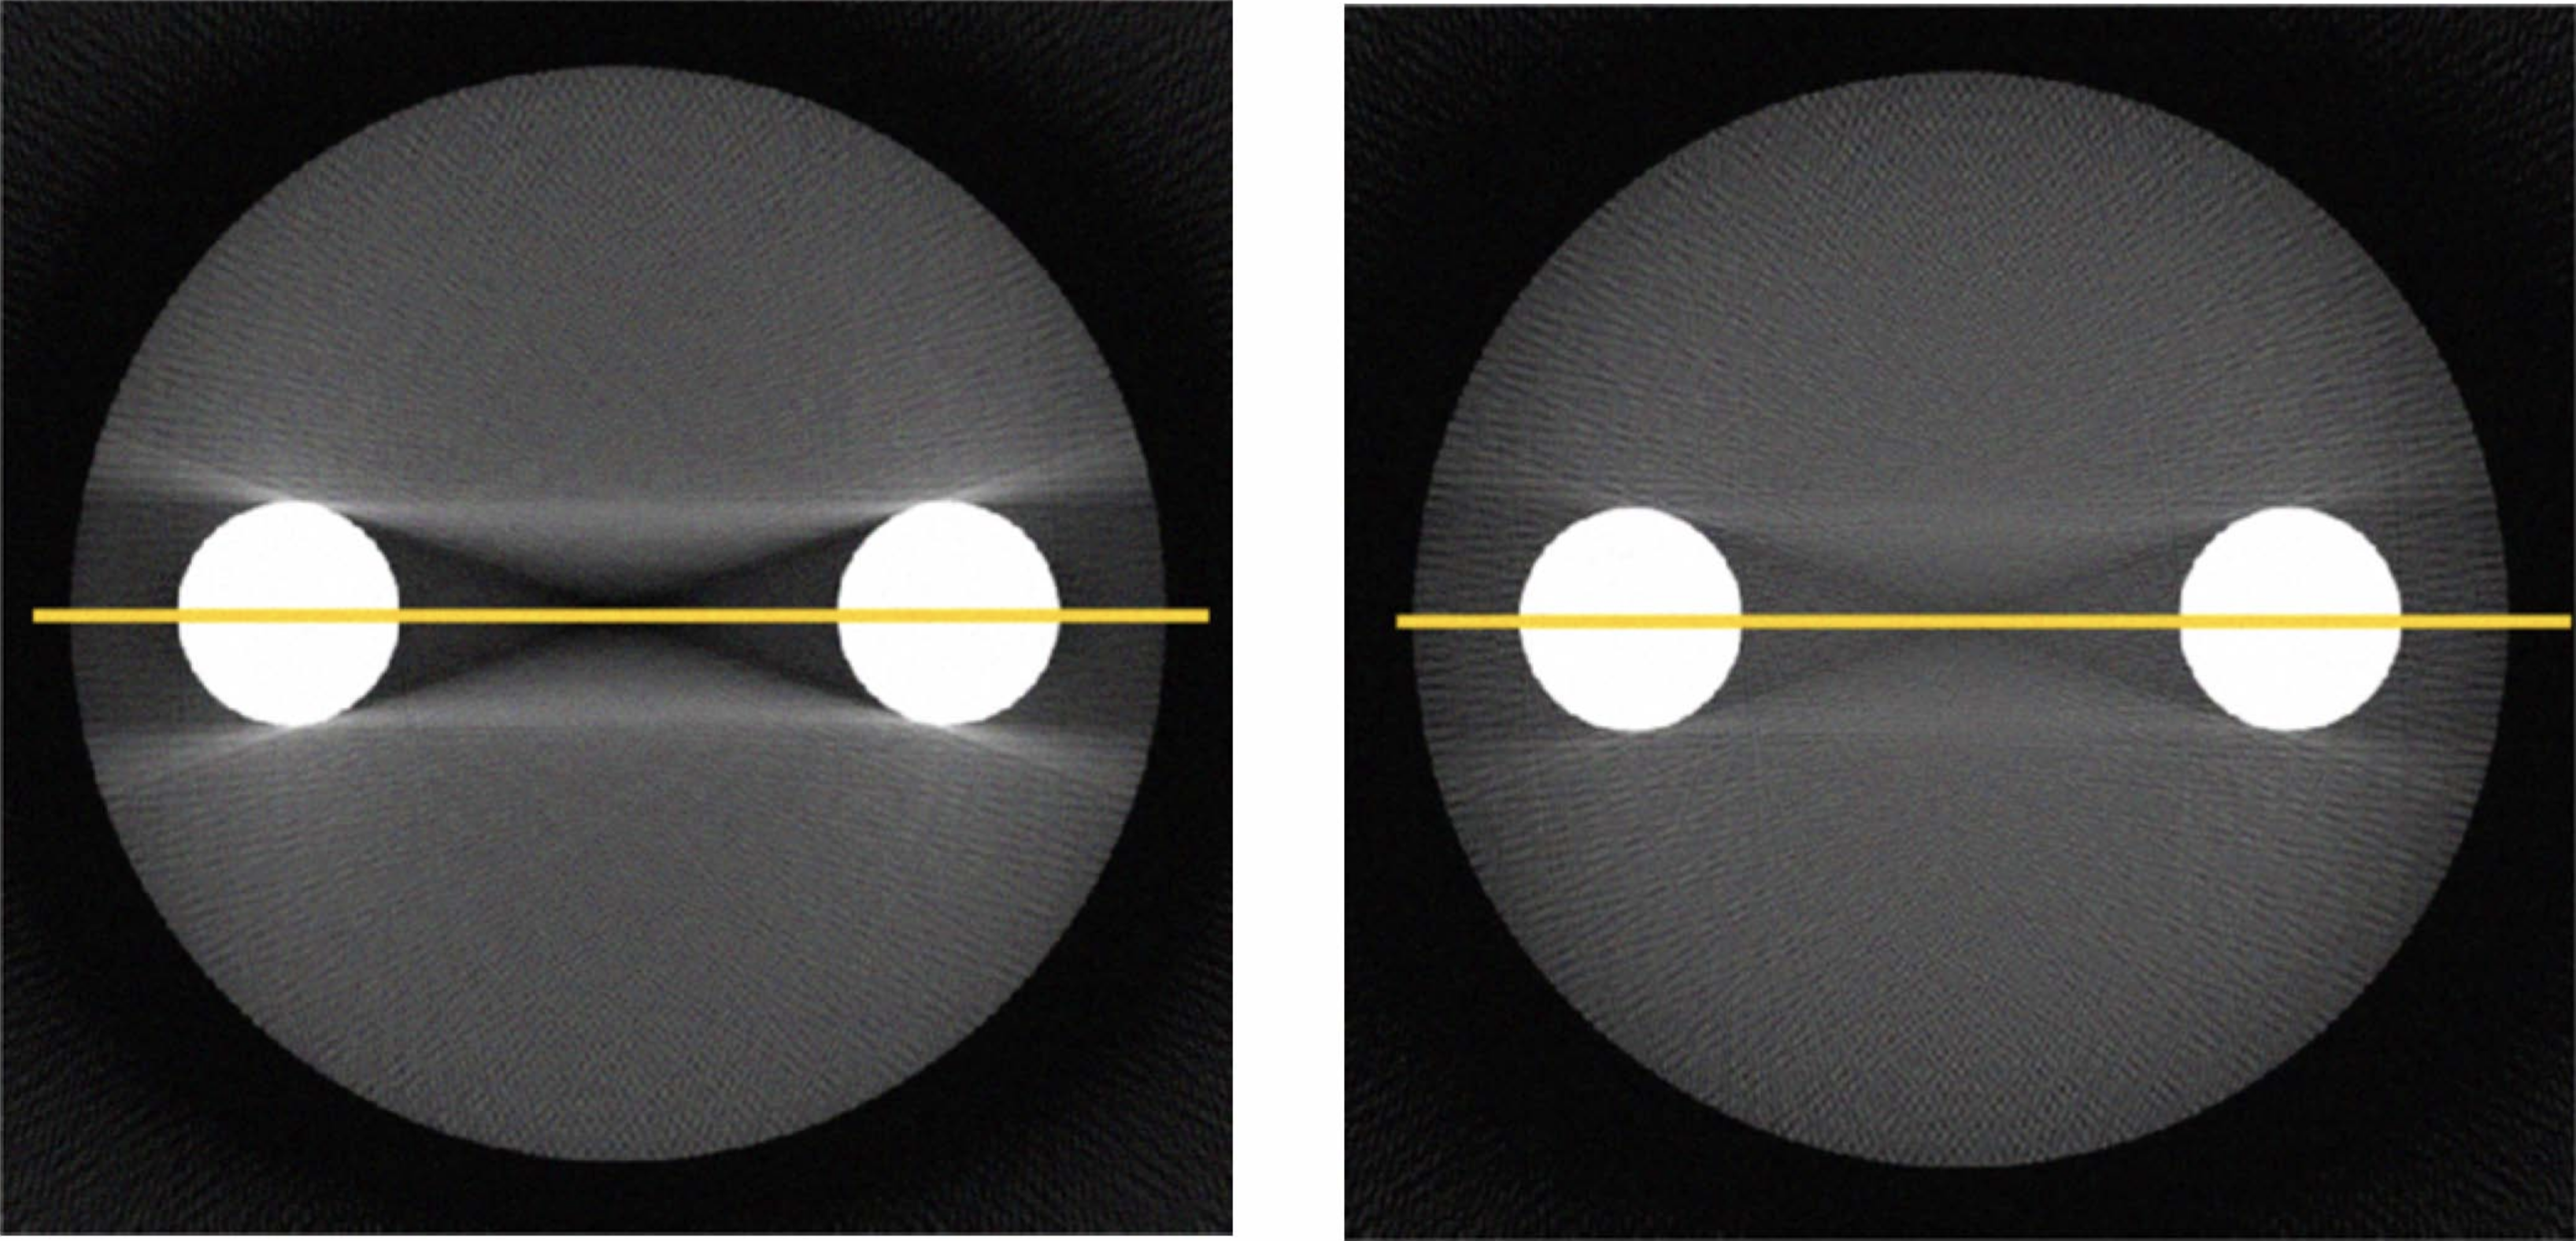
\includegraphics[width=0.8\textwidth]{Figures/mcffd.png}
    \caption{\ac{cbct} of a 70\,mm soft-tissue cylinder with two bone inserts.
    Right: Simulation of a X-ray image with scattering, exibiting typical
    cupping and streak artifacts. Right: Image after scatter correction applying
    \ac{mc} techniques for the simulation of $5 \times 10^6$ photons, showing
    improved uniformity and quantitative accuracy. Right: Image without
    correction, exhibiting typical cupping and streak artifacts. (Figure adapted from \cite{mcffd2011}, \textcopyright 2011 IEEE)}
    \label{fig:scatter_correction_comparison}
\end{figure}


\subsection{Monte Carlo Simulation}

To achieve scatter correction using \ac{mc} simulation, a three-dimensional
phantom is first estimated by analyzing the X-ray projections. Then, an
\ac{mc} simulation is performed to estimate the scatter signal
$I_\text{scattered}$ for each detector pixel. This estimated scatter signal is
then subtracted from the measured intensity $I_\text{measured}$:

\begin{equation}
    \label{eq:scatter_correction}
    I_{\text{corrected}} = I_\text{measured} - I_\text{scattered}
\end{equation}

The \ac{mc} simulation is a powerful computational technique that follows
physics-based principles to model the transport of photons through matter. It is
widely recognized as the gold standard for scatter correction in CT and related
imaging modalities. This status is attributed to several key factors:

\begin{itemize}
    \item \textbf{Physical Accuracy:} \\
        \ac{mc} methods simulate the stochastic nature of photon interactions -
        including Compton and Rayleigh scattering, photoelectric absorption, and
        multiple scattering events - based on fundamental physical
        cross-sections and material properties.

    \item \textbf{Comprehensive Modeling:} \\
        Unlike analytical or empirical methods, \ac{mc} simulations can account
        for complex geometries, heterogeneous materials and realistic X-ray
        spectra, providing highly accurate estimates of the scatter signal.

    \item \textbf{Validation Benchmark:} \\
        Due to their accuracy, \ac{mc}-based scatter estimates are routinely
        used as reference standards for validating and benchmarking faster,
        approximate correction methods.
\end{itemize}


%-------------------------------------------------------------------------------
%	SECTION 4
\section{High-Level Overview of the Monte Carlo Simulation}
%-------------------------------------------------------------------------------

The \ac{mc} simulation of photon transport for scatter correction typically involves the following key steps \cite{mcffd2011}:

\begin{enumerate}
    \item \textbf{Photon Emission:} \\
        Photons are emitted from a virtual X-ray source, with their energies sampled
        from a predefined source spectrum.
        
    \item \textbf{Photon Tracking:} \\
        Each photon is tracked as it propagates through the object. At every
        step, the probability of interaction (either scattering or absorption)
        is determined by the local material properties and corresponding
        interaction cross-sections.
        
    \item \textbf{Interaction Sampling:} \\
        Upon interaction, the event type (e.g., Compton scattering, Rayleigh
        scattering, or photoelectric absorption) and the resulting change in
        photon direction and energy are sampled from the relevant probability
        distributions.
        
    \item \textbf{Detection:} \\
        Photons that reach the detector—either unscattered or after one or more
        scattering events—are recorded. The simulation distinguishes between
        primary and scattered photons, thereby enabling an accurate estimation
        of the scatter contribution at each detector element.
        
    \item \textbf{Statistical Averaging:} \\
        By simulating a large number of photons, the method builds a
        statistically robust estimate of the scatter distribution. The accuracy
        of the result increases with the number of simulated photons and
        ultimately converges toward a stable intensity distribution.
\end{enumerate}

The schematic flow of the Monte Carlo simulation process is summarized in
Figure~\ref{fig:photon-transport-pseudocode}.

\begin{figure}[H]
\centering
\begin{tcolorbox}[colback=white!95!gray, colframe=black!60, width=0.9\textwidth, title=Monte Carlo Photon Transport Algorithm, fonttitle=\bfseries]
\begin{itemize}[leftmargin=1.5em]
    \item \textbf{Initialization:} Define geometry, material composition, and source
    spectrum.
    
    \item \textbf{Loop over photons:}
    \begin{itemize}
        \item Sample the step size to the next interaction point.
        \item Move the photon; check for boundary crossings.
        \item Sample the interaction type; update direction and energy.
        \item If the photon reaches the detector, record the event.
        \item If the photon is absorbed or exits the system, terminate its trajectory.
    \end{itemize}
    
    \item \textbf{Aggregation:} Compute both scatter and primary intensity distributions.
\end{itemize}
\end{tcolorbox}
\caption{Pseudocode representation of the Monte Carlo algorithm for photon transport in scatter modeling.}
\label{fig:photon-transport-pseudocode}
\end{figure}


%-------------------------------------------------------------------------------
%SECTION 5
\section{Monte Carlo Methods: Benefits \& Drawbacks}
%-------------------------------------------------------------------------------

\ac{mc} simulations are widely regarded as the gold standard for scatter
correction in computed tomography due to their ability to model photon-matter
interactions from first principles. These simulations accurately reproduce all
relevant physical scattering phenomena - including Compton and Rayleigh
scattering - and can accommodate arbitrarily complex geometries and
heterogeneous material compositions. Owing to this high degree of physical
fidelity, MC-based methods yield highly accurate scatter estimates and are
commonly employed as reference standards for evaluating and validating
alternative correction approaches.

However, the high accuracy of Monte Carlo simulations comes at the cost of
substantial computational effort. Producing low-noise scatter estimates requires
the simulation of a large number of photon histories to ensure statistical
convergence. Consequently, the runtime scales with the desired level of
accuracy and may range from several minutes to multiple hours or even days,
depending on the complexity of the scene and the available computational
resources. This computational burden poses a major limitation, particularly in
applications involving large datasets or iterative reconstruction workflows.

To address the computational inefficiency of slow-converging \ac{mc}
methods, recent research has explored strategies to accelerate physically
accurate photon transport simulations. Among these, the application of
\ac{qmc} methods has gained increasing attention. By replacing random sampling
with deterministic low-discrepancy sequences, \ac{qmc} techniques can achieve
significantly faster convergence while maintaining comparable accuracy.
Recent \ac{qmc}-based scatter correction algorithms have demonstrated runtime
reductions of multiple orders of magnitude, thereby enabling high-fidelity
simulations even in time-sensitive or resource-constrained environments
\cite{qmcXray2023,lin2025scatter, doignies2024echantillonnage}.

\include{Chapters/Chapter08}
\include{Chapters/Chapter09}
\include{Chapters/Chapter10}
\include{Chapters/Chapter11}

%-------------------------------------------------------------------------------
%	THESIS CONTENT - APPENDICES
%-------------------------------------------------------------------------------

% \appendix % Cue to tell LaTeX that the following "chapters" are Appendices

% Include the appendices of the thesis as separate files from the Appendices folder
% Uncomment the lines as you write the Appendices

% \include{Appendices/AppendixA}
%\include{Appendices/AppendixB}
%\include{Appendices/AppendixC}

%-------------------------------------------------------------------------------
%	BIBLIOGRAPHY
%-------------------------------------------------------------------------------

\printbibliography[heading=bibintoc]

%-------------------------------------------------------------------------------

\end{document}  
